% research-report.tex: 调研报告
% Copyright (C) 2022 吴骏东, 张子辰, 蓝俊玮, 郭耸霄 and 陈建绿
% All rights reserved.

% This file is part of Runikraft. Runikraft is free software,
% which is released under the BSD 3-Clause License, see LICENSE for details.
% Runikraft is provided ``as is'', without any express or implied warrenties.

% The reports of Runikraft are released under the Creative Commons
% Attribution 4.0 International License; see report/LICENSE for details.
\documentclass[UTF8,fontset=none,linespread=1.15]{ctexart}
\ctexset
{
    section/format={\Large\sffamily\bfseries},
    subsection/format+={\sffamily},
    subsubsection/format+={\itshape}
}
\setCJKmainfont[ItalicFont={KaiTi},BoldItalicFont={KaiTi},
BoldItalicFeatures={FakeBold=3}]{Noto Serif CJK SC}
\setCJKsansfont[BoldFont={Noto Sans CJK SC Bold},
BoldItalicFont={Noto Sans CJK SC Bold},
AutoFakeSlant]{Noto Sans CJK SC DemiLight}
\setCJKmonofont[AutoFakeBold=3,AutoFakeSlant]{FangSong}
\setmainfont{cmun}[Extension=.otf,UprightFont=*rm,
ItalicFont=*ti,BoldFont=*bx,BoldItalicFont=*bi]
\setsansfont{cmun}[Extension=.otf,UprightFont=*ss,
ItalicFont=*si,BoldFont=*sx,BoldItalicFont=*so]
\setmonofont{cmun}[Extension=.otf,UprightFont=*btl,
ItalicFont=*bto,BoldFont=*tb,BoldItalicFont=*tx]
%Computer Modern Unicode 的\textasciitilde和\~{}的高度相同,所以用\tildechar表示居中的波浪线~
\newcommand{\tildechar}{\raisebox{-0.35em}{\textasciitilde}}
\usepackage[a4paper,hmargin=1.2in,vmargin=1in]{geometry}
\usepackage{graphicx,tikz,float,multicol,makecell,multirow,longtable}
\usepackage{verbatim}
\usepackage[normalem]{ulem}
\usepackage{CJKfntef}
\usepackage[perpage]{footmisc}

%目录, 参考了OSH-2021/x-sBPF
\usepackage{titletoc}
\titlecontents{section}[2em]{\addvspace{1.3mm}\bfseries}{%
\contentslabel{2.0em}}{}{\titlerule*[5pt]{$\cdot$}\contentspage}
\titlecontents{subsection}[4.2em]{}{\contentslabel{2.5em}}{}{%
\titlerule*[5pt]{$\cdot$}\contentspage}
\titlecontents{subsubsection}[7.2em]{}{\contentslabel{3.3em}}{}{%
\titlerule*[5pt]{$\cdot$}\contentspage}

%图表标题
\usepackage{caption}
\captionsetup{font={sf}}

%代码环境
\usepackage{listings}
\lstset{basicstyle={\normalfont\ttfamily},breaklines,tabsize=4}

\usepackage{enumitem}
\setlistdepth{5}
\renewlist{enumerate}{enumerate}{5}
\setlist{itemsep=0pt,partopsep=0pt,parsep=0pt,topsep=0pt}
\setlist[enumerate,1]{label=\arabic*.}
\setlist[enumerate,2]{label=(\arabic*)}
\setlist[enumerate,3]{label=\textcircled{\arabic*}}
\setlist[enumerate,4]{label=(\textit{\roman*})}
\setlist[enumerate,5]{label=\textit{\alph*})}

\usepackage[colorlinks,unicode,pdfstartview={FitH}]{hyperref}
\hypersetup
{
  pdftitle={2022春 操作系统原理与设计(H) x-runikraft小组 调研报告},
  pdfauthor={吴骏东; 张子辰; 蓝俊玮; 郭耸霄; 陈建绿}
}

%带圈数字,它必须在hyperref之后载入
\usepackage{xunicode-addon}
\makeatletter
\xeCJKDeclareCharClass{CJK}{"24EA, "2460->"2473, "3251->"32BF,"24B6->"24E9,"2160->"217F}
\newfontfamily\EnclosedNumbers{Noto Serif CJK SC}
\AtBeginUTFCommand[\textcircled]{\begingroup\EnclosedNumbers}
\AtEndUTFCommand[\textcircled]{\endgroup}
\makeatother

\makeatletter
\let\textcircled@old\textcircled
\protected\def\textcircled#1{%
	\expandafter\textcircled@old\expandafter{\expanded{#1}}}
\makeatother
\makeatletter
\renewcommand\@makefntext[1]{%
	\setlength\parindent{0.75\ccwd}\selectfont
	\@thefnmark\ #1}
\makeatother
\renewcommand*\thefootnote{\textcircled{\arabic{footnote}}}
\renewcommand{\lstlistingname}{代码}

%上标+引用
\let\nosupcite\cite
\renewcommand*{\cite}[1]{\textsuperscript{\nosupcite{#1}}}

%章节作者
\newcommand{\sectionauthor}[1]{%
\vspace*{-5ex}
\noindent\textrm{\hfill\textit{by #1}}
\vspace*{2ex}\par}
\renewcommand{\today}{2022年4月10日}

\begin{document}
\sffamily %为方便屏幕阅读,文档主要使用无衬线字体
\title{\bfseries Runikraft小组\quad 调研报告}
\author{吴骏东\and 张子辰\and 蓝俊玮\and 郭耸霄\and 陈建绿}
\date{\today}
\maketitle

\tableofcontents

\section{项目简介}
Runikraft 是用Rust语言编写的能在RISC-V架构 + QEMU平台上运行unikernel。
它基于用C语言实现的Unikraft,在继承Unikraft的高效性和可定制性的同时,
进一步简化了构建系统镜像的流程,加入了RISC-V支持,并且
用Rust语言提供了更强的内核安全保证。
\section{项目背景}
\subsection{操作系统的架构}
最初的操作系统缺乏明确定义的结构,也就是简单结构。这类系统的设计者希望用
最小的空间提供尽可能多的功能,因此,系统没有被仔细划分成模块,整个系统是
一个高度耦合的整体,用户程序的错误可能导致整个系统的崩溃。\cite{bib:os-concept}

随着操作系统的
发展,分层系统出现了,这种系统被分割成若干层,最低层为硬件层,最高层为用户
层,每一层都在较低层基础上实现,并为较高层提供一组能调用的程序集。分层系统
简化了构建和调试系统的难度,并且有助于局部优化系统。
然而合理地定义各层并不容易,有时低层组件可能需要
高层组件提供的服务;而且分层会导致用户层执行的操作需要多次转发才能映射到硬件
操作,效率稍差。

随着分层系统的不断发展,系统的内核日益增大,这导致系统的内核愈发难以管理和维护。
微内核就是在这样的背景下诞生的,在这种系统中,只有CPU调度、内存管理、进程通信等
高度依赖特权的模块被放在内核中,而设备驱动、文件系统、网络等系统服务一概是运行
在用户态下的独立服务进程,这些服务进程依靠消息传递机制相互使用。微内核诞生后,原本
的分层系统的内核被称为宏内核。典型的微内核的
代码量在一万行以下,这有助于用形式化方法严格验证内核的正确性,确保内核没有安全漏洞
和功能缺陷。与此同时,运行在用户态下的服务进程之间相对独立,进程的权限恰能提供
相应的服务,一个进程的崩溃不会波及整个系统。所以,微内核系统相比宏内核更安全、
更健壮。虽然与宏内核相比,消息传递会降低系统模块之间的通信效率,但这可以通过共享内存缓解。

受微内核系统的启发,宏内核系统引入了可加载内核模块,即一项服务可以在系统启动后随时链入内核,
或从内核中卸载。
这样,内核的核心组件只需要包含CPU调度、内存管理、进程通信等基本的功能,而其他内核功能可以
根据需要启动。不过,与微内核不同,这些可加载内核模块运行在内核态,它们中的安全漏洞可以
威胁整个内核。\cite{bib:os-concept}

传统上,操作系统应该为用户程序提供尽可能全面的服务,并且要负责在用户程序和系统间、
用户程序之间建立屏障,以防止用户程序的错误影响整个系统。但是,随着计算机的普及,
专为一个用途建造的计算机愈来愈多,这些计算机上只会运行一个用户程序,而这个用户程序
的崩溃也意味着系统的崩溃,所以传统操作系统中的隔离在这种高度专用的计算机中毫无意义,
而消除隔离能减小上下文切换的开销,进而提高效率。当今,需要大量使用专用系统的领域
包括物联网、工业控制和云计算。前两者主要需要实时系统,而后一者与虚拟化密切相关。

\subsection{虚拟化}
在1960s,大型机的运算速度已经远超过了人类的操作速度。为了
充分利用大型机的算力,一台大型机配置了多个终端,多个用户可以同时通过终端与大型机交互,
多个用户的程序轮转使用CPU时间。由于轮转速度很快,用户无法感受到自己的程序没有连续运行,
所以在每个用户看来,他都拥有一台计算机。这种运行在大型机上的分时系统是最初的虚拟化。
然而,随着个人计算机的发展,这种基于分时系统的虚拟化逐渐没落。虚拟化的再次兴起
得益于互联网技术的发展和云计算的兴起,在云计算中,用户通过网络操作远程的虚拟机,
这些远程虚拟机可以向外界提供网络服务。

\subsubsection{虚拟机}
广义上的虚拟机是模拟硬件或解释高级语言的程序,比如Apple在两次macOS架构迁移时
分别推出的Rosetta和Rosetta 2就是硬件模拟器,CPython就是高级语言解释器,
而OpenJDK JRE可以视为硬件模拟器,只不过它模拟的是不存在的硬件。这三个示例
都侧重协助运行程序,而几乎没有隔离措施。狭义的虚拟机是一个模拟完整的计算机系统
的程序,在虚拟机上运行的系统看来,虚拟机和物理机没有明显区别,而且,虚拟机上
运行的系统不能随意访问宿主机的资源,Virtual Box、WMWare就是这类虚拟机。
由于云计算平台上运行的用户程序对计算资源的提供商并不可信,所以,提供商希望将用户
程序与系统的其他部分隔离。这需要狭义的虚拟机。

最初的云计算服务就是向用户提供一台完整的远程虚拟机。通常的远程虚拟机帮助用户提供
网络服务,也就是作为服务器。服务器其实不需要每时每刻都保持运行,而只需要在有人请求这项网络
服务时运行,但是为了确保网络服务的可用性,服务器必须保持开机,用户必须
持续为这台作为服务器的远程虚拟机付费。为了更细粒度地分配计算资源,云计算服务的提供商
推出了serverless服务。在serverless中,原本的服务器被拆分成若干“函数”,其实也就是
一个响应网络请求的程序。当网络服务被请求时,这个程序被启动,响应这个请求,然后退出。
这需要一台虚拟机能够快速启动,可是传统的虚拟机无法满足要求。

\subsubsection{容器}
一种解决方案是不使用虚拟机,而使用更加轻量的方式实现隔离,比如容器。
以Docker为代表的传统容器是为了便捷地打包程序及其依赖诞生的,而并不强调隔离性。
传统容器使用 Namespace/Cgroup 实现,这套容器技术实际上是从进程调度的角度入手,
对内核进行的功能扩展。优势上来说,操作界面很 Linux、很方便,开销也很低,
可以被用来无负担地套在已有应用外面来构建隔离的环境。并且它是纯软件方案,
不和其他层面的物理机、虚拟机相冲突。然而,
随着容器技术的不断发展,传统容器隔离性不足的缺陷逐渐暴露了出来。
Namespace/Cgroup 是内核的一个部分,其中运行的容器仍然使用主机的 Linux 内核,
它解决不了Linux内核中隔离性差的问题,攻击者可以利用Linux内核的漏洞
实现容器逃逸,然后便可以直接对宿主机进行攻击。\cite{bib:docker-security-selinux}

基于操作系统本身的容器机制没办法解决安全性问题,需要一个隔离层。
而虚拟机是一个现成的隔离层,AWS这样的云服务已经让全世界相信,
对用户来说,“secure of VM” 是可以满足需求的。
虚拟机里面只要有个内核,就可以支持 OCI 规范的语义,
在内核上跑个 Linux 应用并不太难实现。所以,安全容器的隔离层让应用的
问题——不论是恶意攻击,还是意外错误——都不至于影响宿主机,
也不会在不同的 Pod 之间相互影响。而且实际上,额外隔离层带来的影响并不仅是安全,
对于调度、服务质量和应用信息的保护都有好处。目前的安全容器有两个主流实现:
\begin{itemize}
\item \href{https://github.com/kata-containers/kata-containers}{Kata Container} 是MicroVM的一个经典的实现,它提供了一个MicroVM,
并且有专门提供给 Kubernetes 的接口,有比较好的安全性和运行效率,
现在已经开始逐步使用。但是其启动时间和内存占用与传统容器还有一定的差距。
\item  \href{https://github.com/google/gvisor}{gVisor} 是
基于进程虚拟化的容器实现,它拥有很好的隔离性,
很小的内存占用和启动时间,但是系统调用效率不高。
\end{itemize}

容器虽然解决了传统虚拟机启动时间长的问题,但是无法兼顾效率和隔离性。

\subsubsection{Unikernel}
Unikernel在MicroVM的基础上更进一步,它放弃了运行在虚拟机上的系统内的隔离,让用户程序
和系统程序运行在同一个地址空间下,用户通过函数调用(如\texttt{call}指令)
而不是软中断或陷入(如\texttt{int}、\texttt{syscall}、\texttt{ecall}等指令)使用
系统提供的服务,这免去了上下文切换的开销,大幅提高了系统调用的效率。
高效的系统调用甚至使unikernel的响应时间和吞吐率优于容器。
由于unikernel本质上是运行在虚拟上
的独立操作系统,它拥有良好的隔离性。Unikernel的系统镜像中只包含了用户程序
需要的代码,这使unikernel的镜像非常轻量,甚至比Docker镜像还小。

然而,为了追求轻量性,
unikernels裁剪了传统的操作系统的众多组件,因此unikernels无法提供许多
常用的库的应用程序接口,所以为了将现有的程序移植到某个unikernel平台,开发者
不得不根据该unikernel的API重构程序。\cite{bib:unikraft}
此外,为了轻量、快速,unikernels
没有启用许多基本的并且不会影响性能的安全措施,这导致unikernels相比容器
更容易受到用户程序的安全漏洞的影响。\cite{bib:unikernel-secuirty}

目前的Unikernel 按实现方式大致可以分为两种:
\begin{itemize}
\item 全新的方式(Clean-slate):在构建单一用途的操作系统的假设下,
自由地使用现代工具来进行构建,比如模块化(modularity)、
声明性代码(declarative code)、避开样板文件(avoiding boilerplate)等。
并且从头开始思考操作系统和应用程序层的实现,
使用高级语言进行系统库的编写,从而使得实现更加可掌控,得到的系统库质量更高。
用 OCmal 语言编写的 MirageOS 就是使用 Clean-slate 方式实现的。
\item 传统的方式(Legacy):在不进行修改或只进行一些小的修改的前提下,
运行现有的软件。这通常通过将现有的操作系统代码库重构到库操作系统中来实现。
用 C 语言编写的 Rumprun 是使用 Legacy 方式实现的。
\end{itemize}

\subsection{Unikernels面临的问题}
Unikernel是为了解决容器的隔离性差和传统的虚拟机启动慢而诞生的,所以unikernels
必须做到启动快、延迟低、吞吐量大。Unikernels的目标是取代容器,成为云计算领域的
最佳选择,所以它们必须提供高效的网络支持。为了方便现有的程序移植到unikernels上,
unikernel应该考虑兼容性问题,它们应该以最小的代价提供目前常用的系统APIs,并且
移植目前常用的库。此外,unikernels镜像的构建不应该过于繁琐。

\subsection{知名的Unikernels}\label{subsec:famous-unikernel-projects}
下面简要介绍我们详细调研了的七个近两年仍然在维护unikernels。

\subsubsection{ClickOS}\sectionauthor{蓝俊玮}

ClickOS 是一个基于 Xen 的高性能的虚拟化软件中间盒平台。为了达到高性能,
ClickOS 对 Xen 的 I/O 子系统实现了广泛的翻修,包括对后端交换机、
虚拟网络设备和后端前端驱动程序。这些更改使 ClickOS 能够显著加快中间盒运行时的网络连接。\cite{bib:12-clickos}

ClickOS 虚拟机只有5MiB ,启动仅需要大约30ms,而且延迟只有45µs。
ClickOS 实现了广泛的中间盒,包括防火墙、运营商级 NAT 和
负载均衡器,并证明 ClickOS 可以每秒处理数百万个数据包,达到生产级性能。\cite{bib:12-clickos}\cite{bib:13-clickos2}

\begin{figure}[!hbt]
\begin{minipage}{0.49\linewidth}
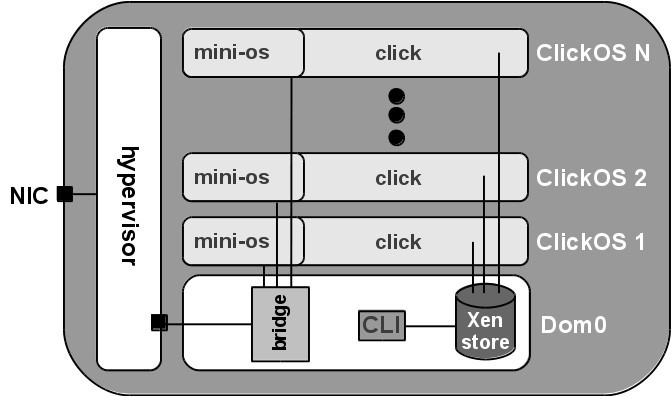
\includegraphics[width=\linewidth]{pictures/clickOS_arch.jpg}
\caption{ClickOS 的架构\cite{bib:13-clickos2}}
\end{minipage}
\begin{minipage}{0.49\linewidth}
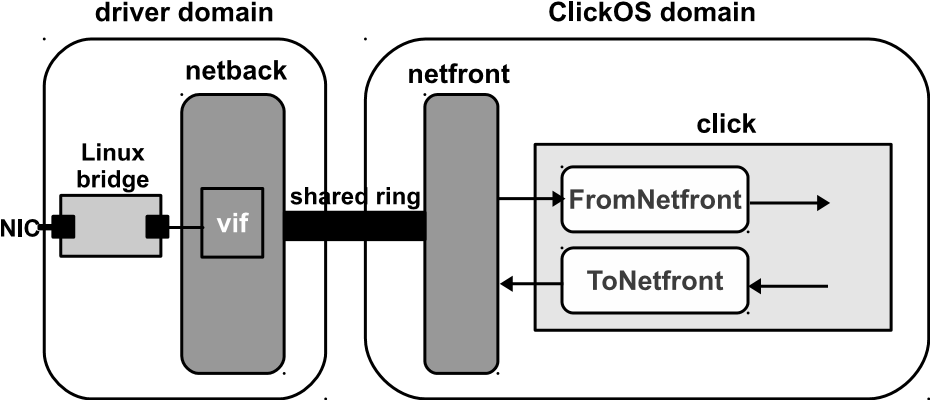
\includegraphics[width=\linewidth]{pictures/ClickOS_networking.png}
\caption{Basic ClickOS networking in Xen\cite{bib:12-clickos}}
\end{minipage}
\end{figure}

\subsubsection{MirageOS}\sectionauthor{蓝俊玮}

MirageOS 是一个用 OCaml 语言编写的,
用于在各种云计算和移动平台构建安全、高性能网络应用程序的库操作系统。
它可以将大型服务器划分为很多更小的虚拟机,使得服务器具有更强的拓展性和安全性。
其代码可以在 Linux 、Mac OS 等系统中开发,然后编译成一个完全独立的、专门的内核,
可以在 Xen、KVM hypervisors 或轻量级 hypervisors 下运行。MirageOS
已经发展成为一个由近100个开放源码库组成的成熟库,实现了一系列广泛的功能,
并且正开始与 Citrix XenServer 等商业产品集成。MirageOS
将 Xen hypervisors当成一个稳定的硬件平台,让我们可以专注于实施高性能协议,
没必要为支持传统操作系统里面的成千上万个设备驱动程序而操心。\cite{bib:11-unikerel2}

\begin{figure}[!hbt]
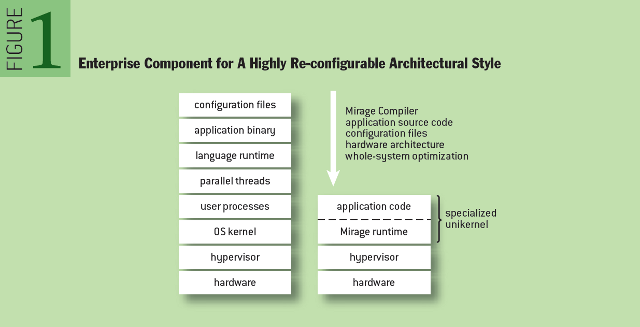
\includegraphics[width=\linewidth]{pictures/figure1.png}
\caption{MirageOS 的架构}\label{fig:mirage-fig1}
\end{figure}

\begin{figure}[!hbt]
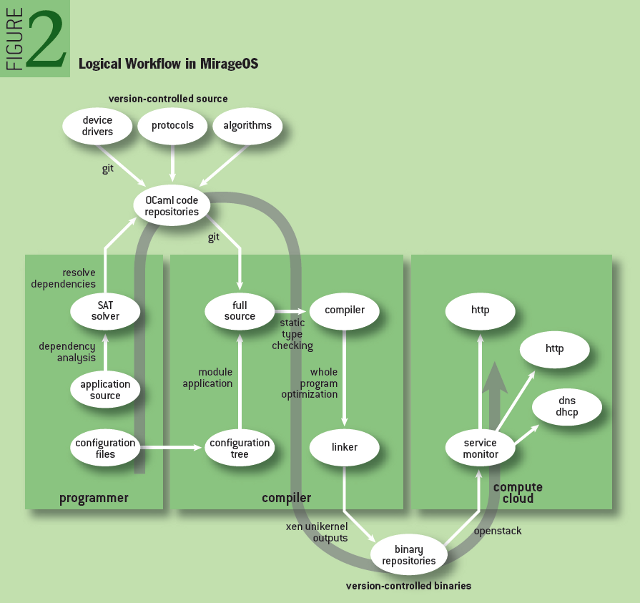
\includegraphics[width=\linewidth]{pictures/figure2.png}
\caption{MirageOS的逻辑工作流}\label{fig:mirage-fig2}
\end{figure}

MirageOS的亮点是输入应用程序的所有源代码依赖项都被显式跟踪,包括实现内
核功能所需的所有库。MirageOS 包括一个构建系统,该系统内部使用
一个 SAT 解算器(使用 OPAM 包管理器,使用 Mancoosi 项目的解算器)
从一个已发布的在线包集中搜索兼容的模块实现。由于 OCaml 的静态类型
检查,在编译时将捕获接口中的任何不匹配。

在 MirageOS 中,OCaml 编译器接收整个内核代码的源代码,
并将其链接到一个独立的本机代码对象文件。它链接到提供引导支持和
垃圾回收器的最小运行时。没有抢占式线程,内核是通过一个 I/O 循环轮询
Xen 设备的事件驱动的。\cite{bib:11-unikerel2}

\subsubsection{IncludeOS}\sectionauthor{蓝俊玮}

IncludeOS 是一个为开发基于 unikernel 的应用程序而创建 C++ API 的项目。\cite{bib:9-includeos}

当 IncludeOS 映像引导时,它通过设置内存、运行全局构造函数、注册驱动程序和中断处理
程序来初始化操作系统。IncludeOS 不支持虚拟内存,应用程序和
 unikernel 库使用单个地址空间。因此,没有系统调用或用户空间的概念; 所有操作系统服务
 都通过对库的简单函数调用来调用,并且都以特权模式运行。\cite{bib:10-includeos2}

\noindent IncludeOS 有如下优点:\cite{bib:9-includeos}
\begin{itemize}
\item IncludeOS中目前没有进程抢占,所以操作系统的行为非常静态。
只要机器本身是可预测的,延迟也将是完全可预测的。因此,在裸机硬件上,
IncludeOS可被视为低延迟,可预测的操作系统。
\item 对网络的支持很好,与 Linux 相比表现出色。
\item IncludeOS 系统作为一个整体进行编译和优化。在编译器和连接器阶段,
优化器可以更多地了解整个系统正在做什么,并且有可能进一步优化。
\item IncludeOS 中的所有 IRQ 处理程序简单地(原子地)更新计数器,
并在有时间时将进一步的处理推迟到主事件循环。这消除了对上下文切换的需要,
同时也消除了与并发相关的问题,如竞争条件。
通过使所有 I/O 都是异步的,CPU 保持忙碌,这样就不会发生阻塞。
\end{itemize}

\noindent IncludeOS 有如下缺点:\cite{bib:9-includeos}
\begin{itemize}
\item IncludeOS 不实现所有 POSIX。开发人员认为,
只有在需要时才会实现 POSIX 的某些部分。开发人员不太可能将完全遵守 POSIX 作为一个目标。
\item 与MirageOS一样,IncludeOS 中没有实现阻塞调用,因为当前的事件循环模型是使用它的最佳方式。
\item IncludeOS 目前还缺少可写的文件系统。
\end{itemize}

\subsubsection{RustyHermit}\sectionauthor{陈建绿}

RustyHermit(\href{https://github.com/hermitcore/rusty-hermit}{Github}) 是
一个基于 Rust 的、轻量级的 Unikernel,也是一个用来评估操作系统新的设计的研究项目。
它用 Rust 语言完全改写了 RWTH Aachen University
 开发的研究项目 \href{http://hermitcore.org/}{HermitCore}\footnote{HermitCore 最初是用 C 语言编写的,是一种针对高性能和云计算的可伸缩和可预测的运行时的 Unikernel。}。\cite{bib:14-rusty-hermit}

该项目完全使用 Rust 语言开发,Rust 的所有权模型保证了它的内存/线程安全,
并且让开发者能够在编译时就消除许多种 bug。因此,与通用编程语言相比,使用 Rust
 进行内核开发会留下更少的漏洞,得到更加安全的内核。

开发者扩展了 Rust 工具链以至于 RustyHermit 的 build 过程
与 Rust 通常的工作流程相似。使用 Rust runtime 而且不直接使用 OS 服务的
 Rust 应用程序能够直接在 RustyHermit 上运行而不需要修改。因此,原则上,
 每一个现有的 Rust 应用程序都可以建立在 RustyHermit 之上。\cite{bib:17-rusty-hermit2}


RustyHermit 中优化实现了网络栈。它使用 \href{https://github.com/smoltcp-rs/smoltcp}{smoltcp}
作为它的网络栈,使用 \href{https://www.linux-kvm.org/page/Virtio}{Virtio}
作为客户机和主机操作系统之间的接口。
%将RustyHermit 和 Linux 分别作为客户端运行在基于 Linux 的主机系统上的虚拟机中,以信息的比特数作为自变量,吞吐量/Mbps作为因变量,
%进行测试并绘图,结果如下:\cite{bib:20-linux-kernel}
%\begin{figure}[H]
%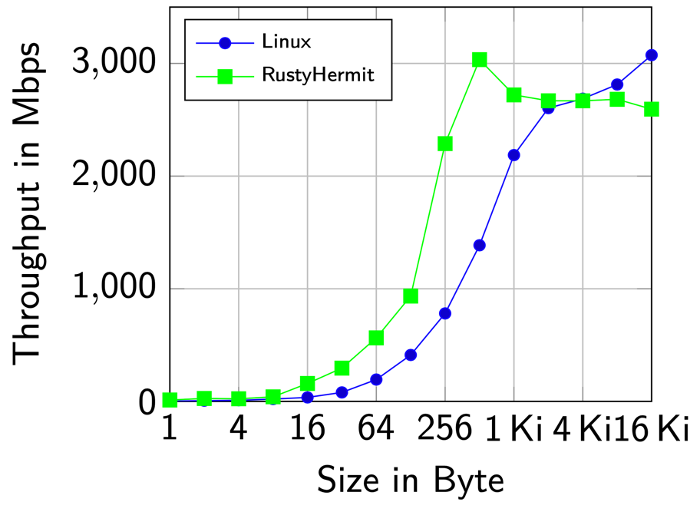
\includegraphics[width=\linewidth]{pictures/RustyHermit-1.png}
%\caption{}
%\end{figure}
%
%由结果图可以看出,\textbf{RustyHermit 在信息比特数较小时吞吐量明显比 Linux 更快}。

Sung, Olivier, Lankes and Ravindran\cite{bib:18-intra-unikernel}
提出了一个修改版本的 RustyHermit,该版本利用Intel MPK(Memory Protection Keys)\cite{bib:19-mpk},
在保持单一地址空间的同时,在 Unikernel 实例中引入内存隔离,
包括安全内核代码与不安全内核代码之间的隔离、内核代码与用户代码之间的隔离。
在一组宏基准测试中,带有隔离功能的 unikernel 仅减慢了0.6\%。

这篇论文中的内容可以作为我们实现 runikraft 的参考。

\subsubsection{Rumprun}\sectionauthor{陈建绿}

Rumprun unikernel 是在 rump kernels 的基础上开发的。
Rumprun 不仅可以在像 KVM 和 Xen 这样的管理程序上工作,
还可以在裸金属上工作。无论有没有 POSIX-y 接口,Rumprun 都
可以正常使用。如果有 POSIX-y 接口,Rumprun 则允许现有的、
未经修改的 POSIX 应用程序开箱即用;如果没有 POSIX-y 接口,
Rumprun 则允许构建高度自定义的解决方案,并且占用的空间最小。

Rumprun unikernel 支持用 C、 C++ 、 Erlang、 Go、
Java、 Javascript (node.js)、 Python、 Ruby 和 Rust 等语言编写的应用程序。

在 \href{https://github.com/rumpkernel/rumprun-packages}{rumprun-packages repository}
中可以找到用于 Rumprun 的现成软件包,比如 \texttt{LevelDB},
\texttt{Memcached}, \texttt{nanomsg}, \texttt{Nginx} 和 \texttt{Redis}。

\paragraph{1. Rump kernels}~

Rump kernels 的组件来自未经修改的 NetBSD,由此开发者提供了一个 POSIX-y API。
Rump Kernel 项目以一种可用于构建轻量级、特殊用途虚拟机的形式提供了 NetBSD 的
模块化驱动程序。因为开发者没有做会将错误引入到应用程序运行时(application runtime)、
libc 或驱动程序中的移植工作,所以程序可以很稳定地工作。\cite{bib:21-rump-kernel}
\begin{figure}[!hbt]
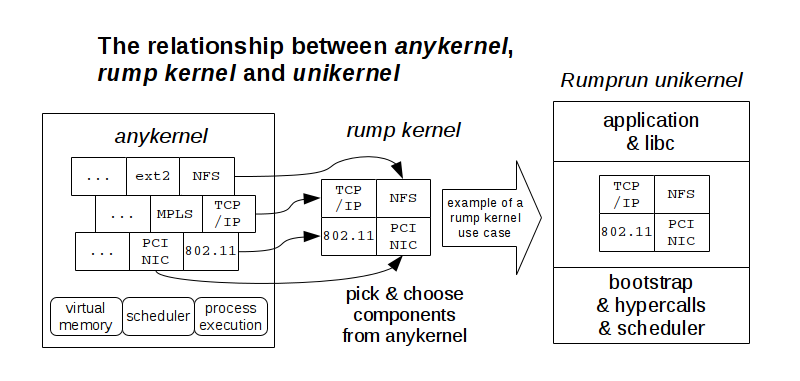
\includegraphics[width=\linewidth]{pictures/rumprun-1.png}
\caption{Anykernel、
Rump kernel 和 Rumprun Unikernel 的关系}
\end{figure}

\begin{quote}
“Anykernel”概念指的是一种与架构无关的驱动程序方法,在这种方法中,驱动程序既可以编译到宏内核中,也可以作为用户空间进程运行,具有微内核风格,并且不需要修改代码。\\
\hspace*{\fill}——维基百科
\end{quote}

\paragraph{2. Rumprun}~

Rumprun 可用于将几乎任何与 POSIX 兼容的程序转换为一个可工作的
Unikernel。使用 Rumprun,理论上可以将 Linux 或者 类Unix系统上的大部分
程序编译成 Unikernel。Rumprun 以开发 NetBSD 内核中的驱动程序并在用户空间
中进行测试的需求为出发点,主要的工作是重构这个代码库,使其看起来像一个库操作系统。\cite{bib:24-rumrun}

\begin{figure}[!hbt]
\begin{minipage}{0.49\linewidth}
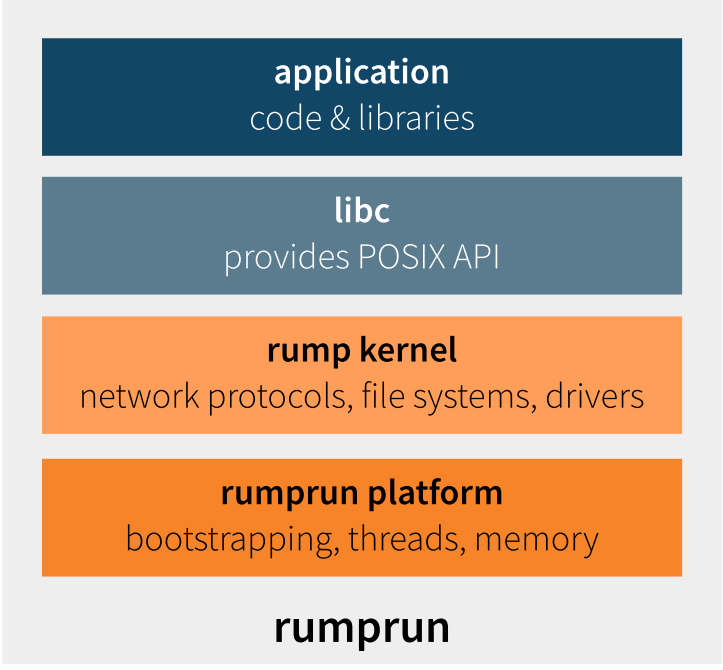
\includegraphics[width=\linewidth]{pictures/rumprun-2-cut.png}
\caption{Rumprun 的架构}
\end{minipage}
\begin{minipage}{0.49\linewidth}
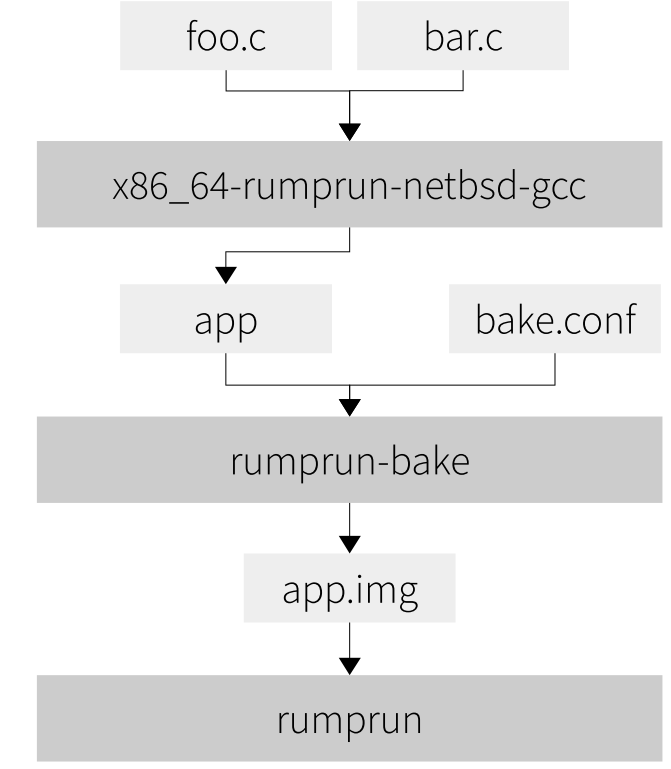
\includegraphics[width=\linewidth]{pictures/rumprun-3-cut.png}
\caption{Rumprun 的工作流程示例}
\end{minipage}
\end{figure}

Rumprun 也有一些限制:

\begin{itemize}
\item single address-space
    \begin{itemize}
    \item no processes
    \item no virtual memory
    \item no signals
    \end{itemize}
\item toolchain
    \begin{itemize}
    \item still experimental
    \end{itemize}
\item threading
    \begin{itemize}
    \item cooperative
    \item single-core
        \begin{itemize}
        \item need to spawn multiple unikernels to use multiple cores
        \end{itemize}
    \end{itemize}
\end{itemize}

我在调研的过程中发现,rump kernel 的好多官方文档都会重定向到
\url{https://rumpkernel.org}这个网址,而这个网址目前只有一些 IT News,
并非和 rump kernel 相关的内容,所以猜测该项目目前已经无人维护。

\subsubsection{Nanos}\sectionauthor{陈建绿}

\href{https://github.com/nanovms/nanos}{Nanos(Github)}一个比较新的正在开发中的 Unikernel。

\begin{itemize}
\item Nanos 是一个新的内核,旨在虚拟化环境中运行一个且仅有一个应用程序。
与 Windows 或 Linux 等通用操作系统相比,它有几个限制——即它是一个单进程系统,
不支持运行多个程序,也不具备通过 ssh 进行用户或远程管理的概念。
\item Nanos 的目标是成为一个比 Linux 安全得多的系统。
它做到这一点的几个依赖:没有用户的概念,每个虚拟机只运行一个进程,限制每个虚拟机中包含的代码数量。
\item Nanos 并不打算在裸金属上运行,所以开发者努力使其内核\textit{尽可能简单}。
\end{itemize}

%这也许会对我们的项目有所帮助。

\subsubsection{Unikraft}\sectionauthor{张子辰}
Unikraft是一个比较新的unikernel。它在设计时就充分考虑
了现有的unikernels的优缺点。它在保持unikernel的极简化、
高效的同时,兼容了完整的POSIX兼容层,使开发者可以轻松地将现有的为Linux
编写的代码移植到unikernel上。Unikraft由若干低耦合的模块组成,内存分配器、
调度器、网络栈、引导代码都是独立的微型库。Unikraft的API即为微型库本身,
这意味着可以在生成时轻松地添加或移除APIs。\cite{bib:unikraft}

Unikraft遵从如下设计原则:
\begin{itemize}
\item 内核应该是完全模块化的,以便允许unikernel被彻底而轻松的定制。
在Unikraft中,内存分配器、调度器、网络栈、引导程序等系统原件都是
独立的微型库。
\item 内核应该提供注重效率、良定义的API,而且允许用户轻松地
为了满足自己的程序的性能要求选择、组装它们。在Unikraft中,这些APIs
就是微型库本身,这意味着它们可以轻松地在构建时增减,而且提供更多
的微型库即可拓展它们功能。
\end{itemize}

目前,Unikraft已经支持SQLite, nginx, Redis等程序,C/C++, Go, Python, Ruby,
Web Assembly and Lua等编程语言或运行环境。

在架构方面,Unikraft融合了宏内核的单地址空间带来的高效性和微内核的模块化带来的
可拓展性。OS的功能被分割成若干细粒子度的组件,而各个组件之间通过良定义的APIs
通信。Unikraft用精心设计的APIs和静态链接获得高效率,而不是为了效率破坏API
的边界。Unikraft大致分为两部分:
\begin{description}
\item[微型库]微型库是实现一部分的Unikraft的APIs的软件组件,
Unikraft的作者有意将它们分割到了不同的库中,并尽可能降低它们之间的依赖。
实现相同APIs的微型库可以相互替换。比如,Unikraft内核就提供了多种实现
\texttt{ukalloc}接口的内存分配器。
\item[构建系统]它为用户提供基于Kconfig的配置菜单\footnote{在实验1中,
我们在定制Linux内核时,运行\texttt{make menuconfig}后看到的就是Kconfig菜单。},
用户可用它选择要用哪些微型库,要为哪个平台和哪个CPU架构构建。
\end{description}
\begin{figure}[!hbt]
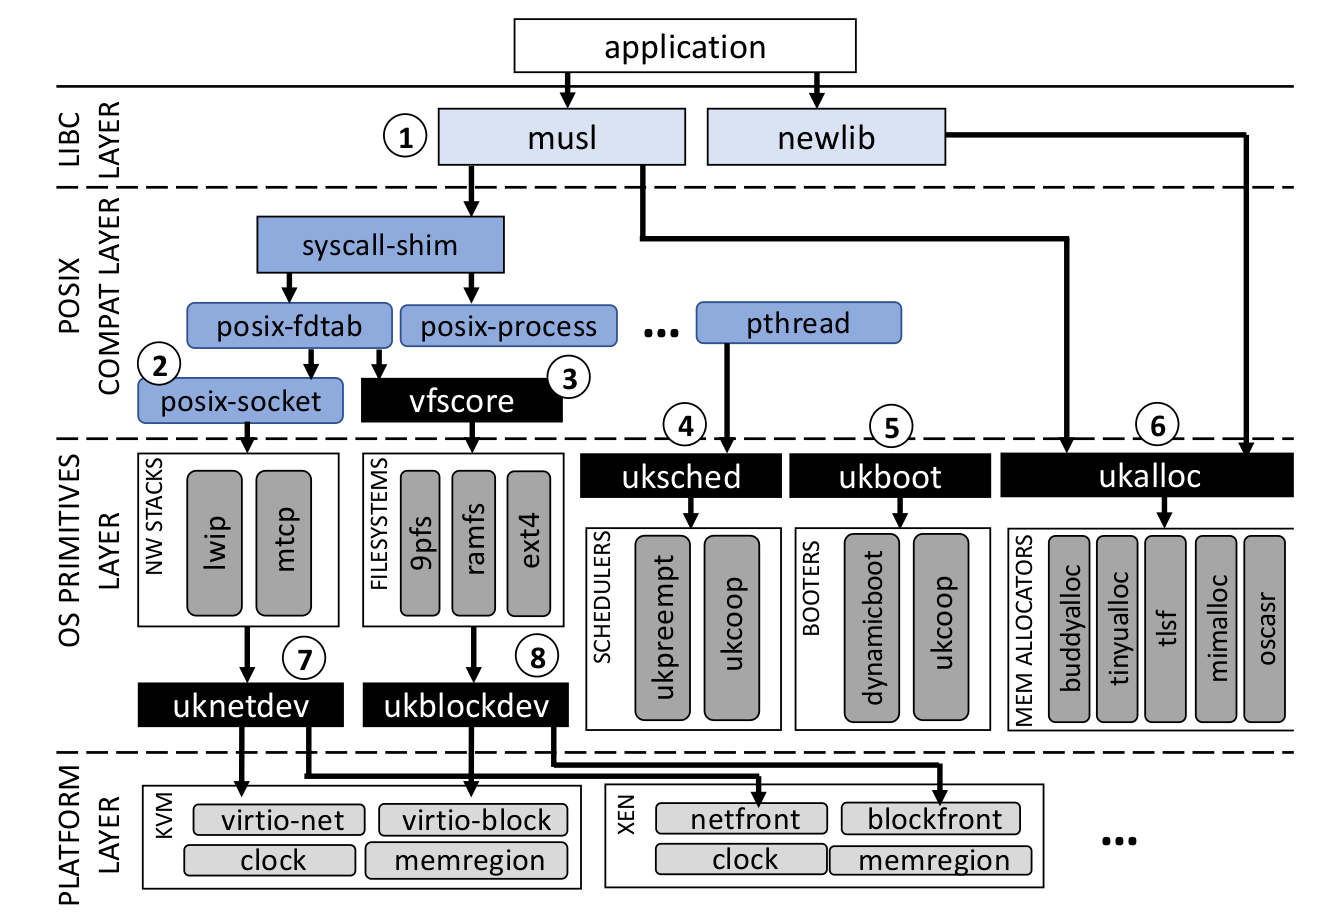
\includegraphics[width=\linewidth]{pictures/Unikraft-architecture.png}
\caption{Unikraft的架构(黑色框内的是APIs)允许用户程序接入不同层次的APIs,也
允许用户选择不同的API实现。}\label{fig:unikraft-arch}
\end{figure}

图\ \ref{fig:unikraft-arch}\ 展示了Unikraft的架构。使用不同层次的APIs和
替换API实现的能力给开发者提供了多种优化可能。首先,未经修改的程序(如用C语言
写的Hello World和nginx)可以使用\texttt{musl}(图\ \ref{fig:unikraft-arch}\ 的①)
或\texttt{nolibc}提供的POSIX兼容层,并自动获得低启动时间、低内存消耗和
更高的吞吐量,因为在Unikraft中,系统调用是高效的函数调用。

类似地,程序的开发者可以轻松选择合适的内存分配器(⑥)以达到最高效率,甚至
在同一个unikernel中使用多种分配器。

关注快速引导的开发者也可以使用自己的遵守\texttt{ukboot} API的引导代码(⑤)。
对于网络密集型程序,开发者可以使用标准的套接字接口(②),或者使用更底层、更高效
的\texttt{uknetdev} API(⑦)以便大幅提高吞吐量。

类似地,数据库这样的硬盘密集型程序可以使用标准的\texttt{vfscore}微型库(③),
或者用\texttt{ukblock} API提高吞吐量(⑧)。

调度器也是可以插拔的(④),而且每个CPU核可以运行不同的调度器。


与其他unikernels相比,Unikraft的系统镜像更小、运行所需内存更小、吞吐量更大:
\begin{figure}[H]
\centering
\begin{minipage}{0.32\linewidth}
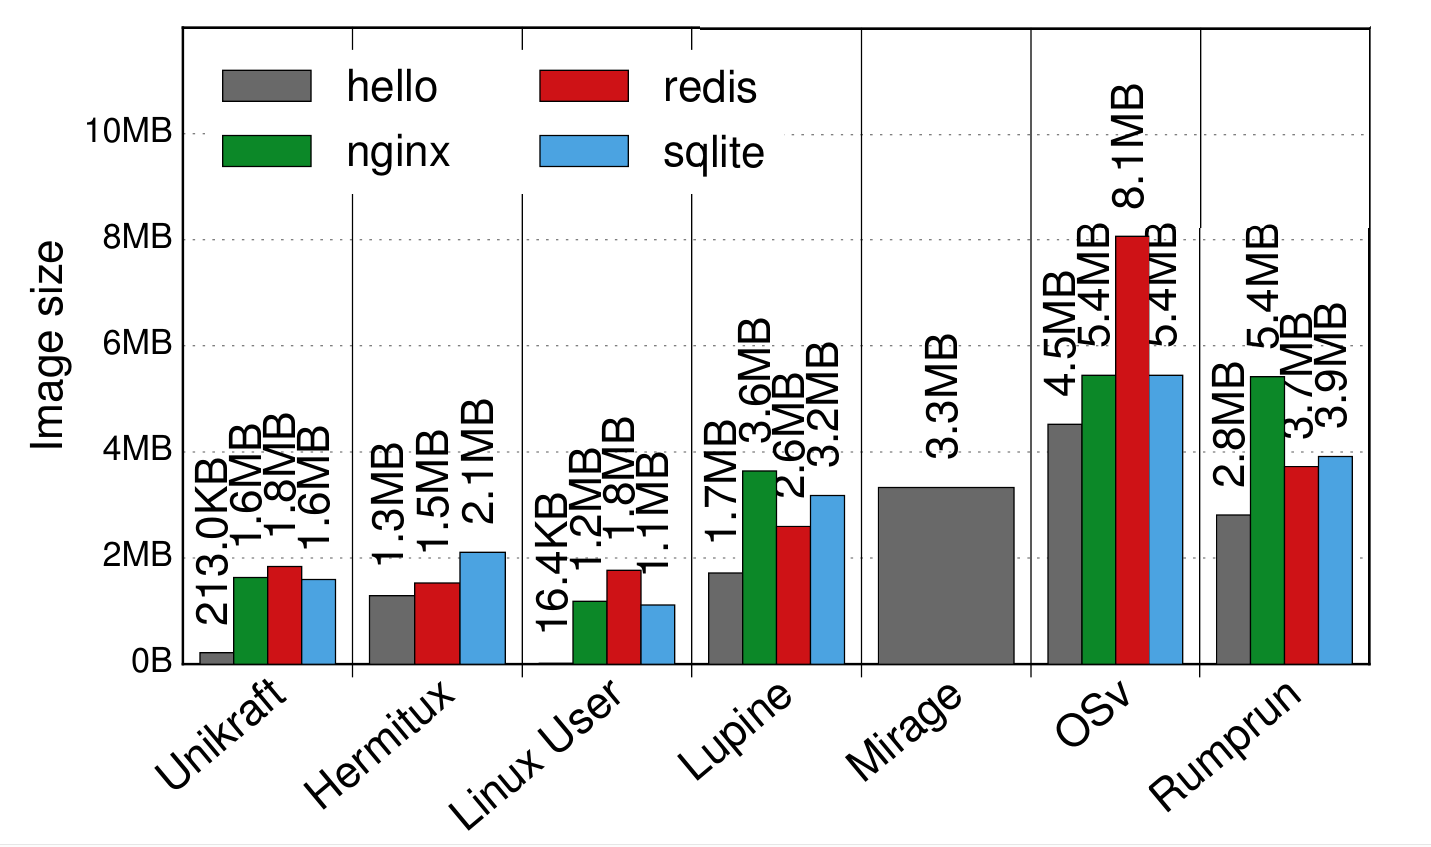
\includegraphics[width=1\linewidth]{pictures/Unikraft-image-size.png}
\caption{}
\label{fig:unikraft-image-size}
\end{minipage}
\begin{minipage}{0.32\linewidth}
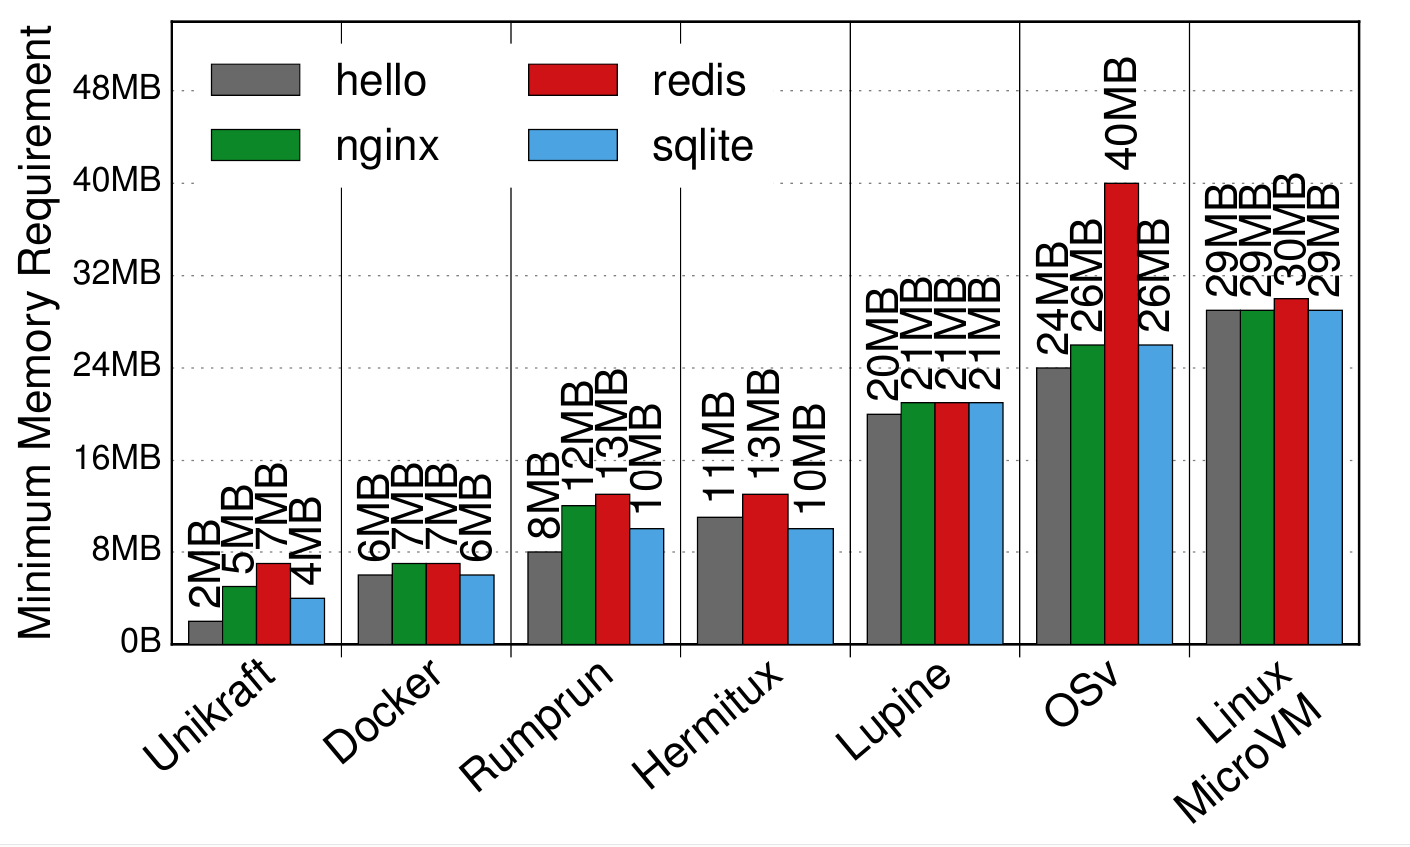
\includegraphics[width=1\linewidth]{pictures/Unikraft-memory.png}
\caption{}
\end{minipage}
\begin{minipage}{0.32\linewidth}
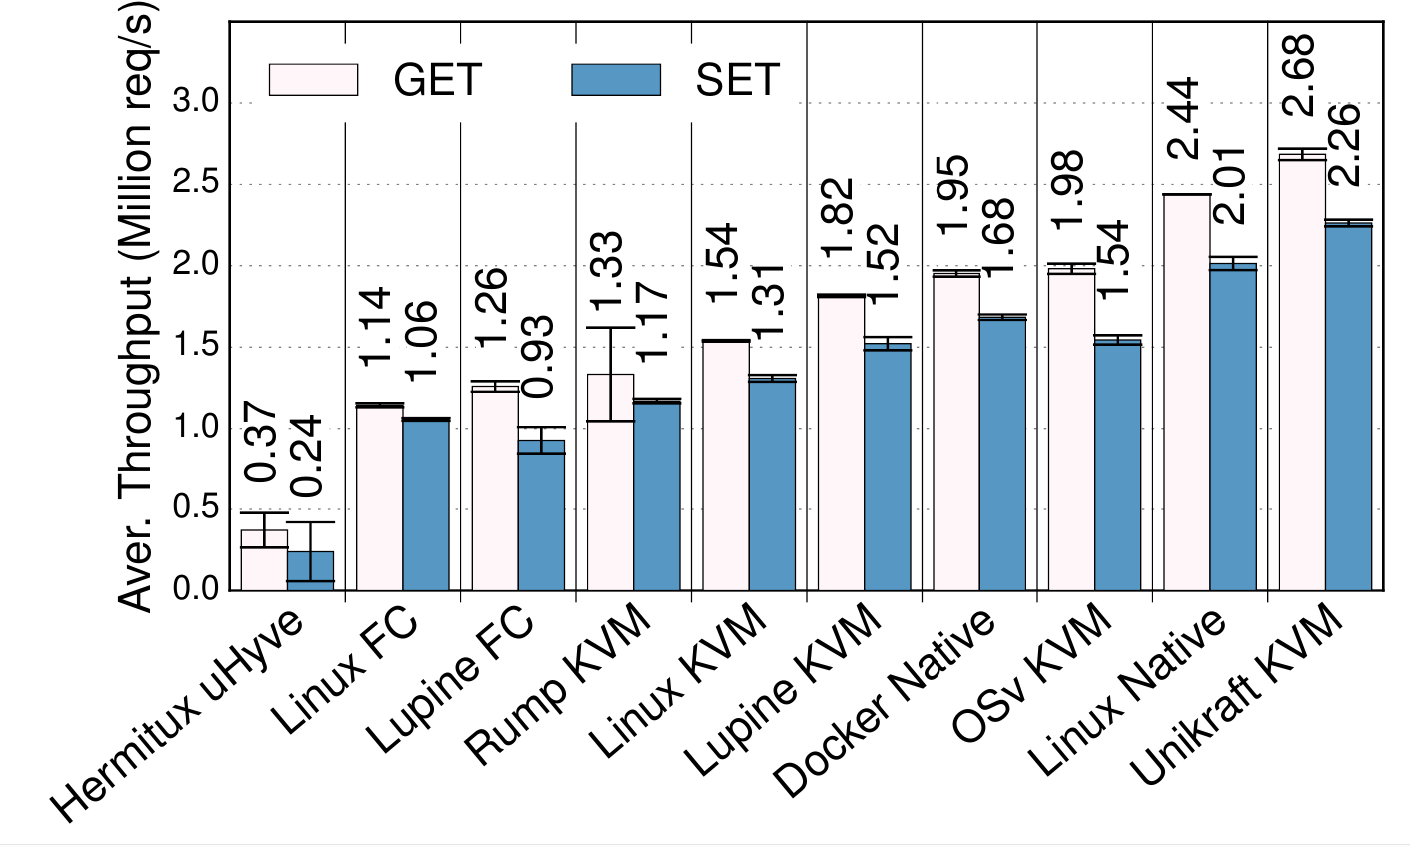
\includegraphics[width=1\linewidth]{pictures/Unikraft-throughput.png}
\caption{}
\end{minipage}
\end{figure}

Unikraft在提升效率的同时兼顾了安全性。根据NCC Group\cite{bib:unikernel-secuirty},
虽然 unikernel 相比容器体积更小、隔离性更好,但是由于不存在内核态-用户态隔离,
且缺乏W\^{}X、stack canary等安全特性,unikernel 其实比传统的容器更不安全。
也就是说,攻击者可以利用 unikernel 上的程序的漏洞,控制 unikernel 所在的虚拟机,
进而未经授权访问资源。
%以 unikernel 的传统应用领域云计算为例,
%如果某个 unikernel 负责处理用户的敏感数据——它通过网络获取用户的数据,
%然后将计算结果通过网络发回,则它一定拥有读用户数据的权限。那么,
%一旦这个 unikernel 存在安全漏洞,攻击者虽然不能控制 unikernel 所在的宿主机,
%但足够窃取用户的数据。
所以,不能片面地把安全性与隔离性等同。而且我们不能
片面地认为使用 Rust 这样的安全的程序设计语言就能保证安全,
因为完整的 unikernel 上不只包含安全的系统代码(或者说库代码),还包含可能不安全的用户代码,
而后者可以导致整个系统不安全。因此,要实现安全的 unikernel,不能仅仅依靠安全的程序设计语言,
而需要额外的安全特性。

NCC Group提到了ASLR、分页保护(如W\^{}X政策、内部数据加固、保护页、空页面漏洞等)、
栈保护标志\footnote{它的英文stack canary来自金丝雀曾经被用来检查煤矿的有毒气体的典故\cite{bib:canary}。}、堆加固、标准库加固等安全措施。
%\begin{itemize}
%\item 地址空间布局随机化 (ASLR)。
%\item 分页保护:如W\^{}X政策、内部数据加固、保护页、空页面漏洞。
%\item 栈保护标志(stack canary,典故:金丝雀曾经被用来检查煤矿的有毒气体\cite{bib:canary}):在栈的返回地址后加上一个随机的整型变量(canary),执行\texttt{ret}前检查 canary 是否被修改。
%\item 堆加固:堆的结构通常是双向链表,链表的元数据(如指针)通常与数据块相邻,堆上的溢出可以改变这些数据块,导致内存的分配、释放算法出错,通常的加固方法是为元数据增加校验值。
%\item 熵和随机数生成器:通常的 unikernel 缺乏足够产生密码学安全的伪随机数的硬件熵,这导致 unikernel 上生成的伪随机数的质量差,解决方法有使用 CPU 的专用随机数指令(如 x86 的 \texttt{rdrand})
%\item 标准库加固:如\texttt{printf} 的 \texttt{\%n} 格式符、自定义格式符、\texttt{\_FORTIFY\_SOURCE} 宏。
%\end{itemize}
它测试了 rumprun 和 includeOS 两个 unikernels,并发现它们几乎没有实现任何安全特性。

尽管 Unikraft 使用 C 语言实现,但它支持(或计划支持)
\href{https://github.com/unikraft/unikraft/tree/staging/lib/uksp}{Stack SP}、
\href{https://github.com/unikraft/unikraft/tree/staging/lib/ubsan}{UBSAN}、
\href{https://github.com/unikraft/unikraft/pull/421}{ARM BTI}、\href{https://github.com/unikraft/unikraft/pull/191}{KASAN}、\href{https://github.com/unikraft/unikraft/pull/239}{PIE}、True Random Number Generator、
Intel CET、ARM SB等安全特性。\cite{bib:unikraft-secuirty}

%总的来说,Unikraft是我们发现的最好的unikernel项目,所以我们的项目将
%主要参考它。

\subsubsection{比较}
表\ \ref{table:unikernel-compare}\ 比较了我们详细调研的unikernels。因为现有的
资料并没有包含我们需要的所有信息,表中的一些信息是依靠阅读源代码获取的。
\small
\begin{longtable}{|c*{7}{|>{\centering\arraybackslash}p{0.095\linewidth}}|}
\caption{Unikernels的比较}\label{table:unikernel-compare}\\
\hline
&ClickOS&\resizebox{\linewidth}{\height}{MirageOS}&\resizebox{\linewidth}{\height}{IncludeOS}&\resizebox{\linewidth}{\height}{RustyHermit}&Nanos&Rumprun&Unikraft\\\hline
\endhead
实现语言&C++&OCaml&C++&Rust&C&C&C\\\hline
支持架构&x86-32、x86-64&x86-64、ARM-64&x86-32、x86-64、ARM-64&x86-64、ARM-64&x86-64、ARM-64、RISCV-64gc&x86-32、x86-64、ARM-64&x86-64、ARM-32、ARM-64\\\hline
支持平台&Xen&KVM、Xen&KVM、Virtual Box、VMWare、x86物理机&QEMU、Uhyve&众多,包括但不限于Xen、KVM、WMWare、Virtual Box等&Xen、嵌入式设备&KVM、Xen、Solo5、Linux用户态\\\hline
支持语言&C、C++&OCaml&C、C++&Rust、C、C++、Go、Fortran&众多,包括但不限于C、Go、PHP、Node、Ruby、Lua、Perl等,理论上支持任何ELF文件&众多,包括但不限于C、C++、Erlang、Go、Java、Javascript (node.js)、Python、Ruby 、Rust等&众多,包括但不限于C、C++、Go、Python、Ruby、Web Assembly、Lua等\\\hline
构建系统&Click configuration language&Opam&Conan、CMake&cargo、CMake&系统与用户程序分别构建,系统使用Makefile构建&buildrump&Kraft、Kconfig\\\hline
安全性&不详&用安全语言实现,支持random device&较差,甚至关闭了一些C++编译器支持的安全特性&
用安全语言实现,支持堆栈保护、应用程序堆栈与操作系统库堆栈分离,有支持页保护的衍生作品&支持ASLR、页保护&有限,\texttt{.text}段不可写,有一定的堆保护,默认引入大量无用库&支持Stack SP、UBSAN、ARM BTI、PIE、Intel CET、random device等安全特性\\\hline
API&专用API&OCaml标准库,和大量其他用OCaml实现的库&不完整的C、C++、POSIX API支持&Rust标准库,部分C、C++、Go、Fortran API&无,依靠系统调用与用户程序通信&C、POSIX API和大量软件包,默认开启系统调用&专用API、POSIX API、C API和众多库\\\hline
网络&有&有&有&用smoltcp实现&有&有&可选择lwip和mtcp两种实现\\\hline
内存管理&有&有,支持垃圾回收&有&有&有&有&有,可以选择多种分配器\\\hline
线程管理&有&无抢占,有进程通信支持&有&有,支持优先级&有&无抢占&支持抢占和无抢占两种调度器,有进程通信支持\\\hline
文件管理&无&支持FAT和mmap&支持mmap和读FAT32&可以支持多种文件系统后端,目前支持virtio-fs和mmap&有&有&支持9pfs和mmap\\\hline
备注&基于MiniOS&&&&相比unikernel,Nanos更像一个微型内核&包含大量NetBSD的代码&\\\hline
\end{longtable}
\normalsize

%\subsection{Unikernels面临的问题}

\section{立项依据}\sectionauthor{张子辰}
我们调研的unikernel项目的不足之处可以概括为(并不每个unikernel都有所有缺点):
\begin{itemize}
\item 系统内的组件耦合度过高,系统不易裁剪或拓展。在拓展方面做得比较好的unikernels有
MirageOS、Rumprun和Unikraft。
\item 需要使用专用的工具构建系统镜像。对于只有几个源文件的小型项目,使用专用的工具并不
是什么大问题,但是,对于由成千上万个源文件组成的大型项目,更改构建环境本身就是一项浩大
的工程。目前,Nanos允许用户程序使用独立的工具构建,MirageOS和RustHermit的构建工具
是它们的语言的默认工具。
\item 将安全性与隔离性等同,忽视了单个unikernel虚拟机的安全。目前,在文档中明确提到
安全措施的unikernels有RustyHermit、Nanos和Unikraft。
\item 核心代码使用不安全的程序设计语言编写。使用安全的编程语言写的unikernels只有MirageOS和
RustyHermit。用不安全的程序设计语言难以避免实现时引入的安全漏洞。
\item 不支持RISC-V架构。目前只有Nanos支持RISC-V架构。
\end{itemize}
虽然说兼容性也是unikernels的一大不足,但是许多unikernels的开发者已经在尽力解决
它,以至于除了MirageOS外的unikernels都提供了或多或少的C标准库支持。

Nanos在兼容性、易构建性方面做得都很好,也支持RISC-V架构,可是它似乎为了支持
直接运行ELF文件,抛弃了unikernels的最重要的无系统调用的特性;Unikraft声称可
配置为POSIX兼容,而且系统架构比较清晰,可惜它不支持RISC-V,而且镜像的构建需要专用
工具。Nanos和Unikraft的共同缺陷是使用不安全的C语言编写。MirageOS使用安全的语言编写,
并且有丰富的软件包资源,可是完全不支持现有的程序;想将程序移植到MirageOS上必须用OCaml
重构程序。RustHermit是对用C语言实现的HermitCore的重构,我们受它的启发,也决定用Rust
重构一个现有的unikernel。

我们小组计划仿照Unikraft的架构,用Rust语言编写能在RISC-V架构+ QEMU平台上
运行的unikernel——Runikraft。Runikraft的核心代码使用Rust编写,但
允许用户代码使用任何语言编写
%——只要它能够被编译成入口为\texttt{\_start}的目标代码
。Runikraft强调构建系统镜像的简洁,用户只需要
修改现有的项目的编译参数就可以构建基于Runikraft的系统镜像,而不必使用
专用的工具链,更不需要重构代码。具体的方法是先将Runikraft编译成静态库,
然后通过修改编译参数,让用户程序不链接标准库,而链接到Runikraft。

Runikraft支持内存管理、进程调度、
进程通信和磁盘管理,而且这些功能都是是可选的且可
拓展的,如果用户不需要某项功能,他可以不将相关模块打包进系统镜像中,
如果用户能够提供某些功能的更好实现,他可以用自己的实现替换原有的模块。

Runikraft的亮点:
\begin{itemize}
\item 用安全的Rust语言编写;
\item 支持正在迅速发展的RISC-V指令集架构;
\item 构建流程简单;
\item 模块化设计,在保持unikernel的高效的同时降低维护难度。
\end{itemize}

Runikraft的目标是提供比较完整的POSIX兼容层、Linux兼容层和C标准库,
但是考虑到时间有限,这些功能只能部分实现。

%如果时间允许,我们还会尝试:
%\begin{enumerate}
%\item 支持更多架构,比如目前流行的AMD64和ARMv8;
%\item 支持在裸机上运行,虽然unikernel为云计算诞生,但这并不代表它只适合
%    云计算领域,事实上,任何专一用途的设备上的系统都可以是unikernel,
%    而且unikernels理论上可以具有比现有的实时系统更高效率;
%\item 支持调试,zos小组\textsuperscript{\ref{ssubsec:x-zos}}曾做过相关研究;
%\item 移植更多库。
%\end{enumerate}

我们考虑过改善unikernel的调试,即zos小组的研究,
但是我们发现,QEMU事实上已经支持交互式的虚拟机调试了。

我们考虑过但最终不打算实现与Linux的二进制兼容,即
unipanic小组的研究,因为
我们认为不会出现需要移植无法获得源代码的程序的情况:
\begin{itemize}
\item 如果源代码因著作权问题无法获取,
    \begin{enumerate}
    \item 修改二进制文件移植,即把\texttt{syscall}指令替换为\texttt{jmp}
    指令后移植。这样可以保持效率,但会侵犯著作权。
    \item 直接移植未修改的二进制文件。这需要\texttt{syscall},会引入上下文切换
    开销,效率难以保证。
    \end{enumerate}
\item 如果源代码因软件无人维护无法获取,那这样的过时软件本身就不应该被继续使用。
\end{itemize}

在系统架构方面,我们将主要参考Unikraft;
在技术方面,我们将参考RustyHermit、Nanos和Chen and Wu的\textit{rCore Tutorial Book}\cite{bib:rcore-os}。

\begin{comment}

\subsection{Unikernel}
Unikernel是专一用途的、单地址空间的轻量操作系统。Unikernels在虚拟机
上运行时,能够提供比传统的容器更短的启动时间、更高的运行效率和更强的
隔离性,因rn此unikeels通常被用在云计算领域。\cite{bib:unikernel}


\noindent 现有的unikernels普遍存在以下问题:\cite{bib:unikraft}
\begin{itemize}
\item 编译它们并让它们达到高效率需要大量专业的工作,而且这些工作通常
需要对每个目标应用程序重做。
\item 它们通常不是POSIX兼容的,需要移植程序和语言环境。
\end{itemize}

\ref{subsec:famous-unikernel-projects}\ 小节将简要介绍我们小组详细调研的ClickOS、MirageOS、IncludeOS、Rusty-Hermit、Rumprun
和Unikraft等六个目前仍然在维护的unikernel项目。
\end{comment}

\section{前瞻性/重要性分析}

\subsection{使用先进的工具构建}

Rust和RISC-V都是新兴事物,它们都是在吸取旧事物的教训的基础上诞生的,
而且,实践表明,两者都正在经历蓬勃的发展,并正在分别逐步取代旧事物。
%而unikernel本身也是比较新颖的操作系统结构,它在云计算领域正在逐步取代
%传统的容器,并且有在嵌入式领域取代传统的嵌入式实时系统的潜能。
因此,用Rust在RISC-V上开发unikernel顺应了历史的趋势。

Rust 是由 Mozilla 研究室
主导开发的一门现代系统编程语言,自 2015 年 5 月发布 1.0 之后,一直以每 6 周
一个小版本的开发进度稳定向前推进。语言设计上跟 C++ 一样强调零开销抽象和 RAII。
拥有极小的运行时和高效的 C 绑定,使其运行效率与 C/C++ 一个级别,非常适合对性能
要求较高的系统编程领域。利用强大的类型系统和独特的生命周期管理实现了编译期内存管理,
保证内存安全和线程安全的同时使编译后的程序运行速度极快,Rust 还提供函数式编程语言
的模式匹配和类型推导,让程序写起来更简洁优雅。\cite{bib:2-why-rust}
总地来说,Rust是一门赋予每个人 构建可靠且高效软件能力的语言。\cite{bib:1-rust-lang}
Rust具有高性能、可靠性、生产力三方面的优势。

RISC-V是于2010年诞生自加州大学伯克利分校的精简指令集架构,
它的目标是成为一个通用的指令集架构,它能适应包括从最袖珍的嵌入式控制器,
到最快的高性能计算机等各种规模的处理器;它能兼容各种流行的软件栈和编程语言;
它能适应所有实现技术,包括现场可编程门阵列(FPGA)
 、专用集成电路(ASIC) 、全定制芯片,甚至未来的设备技术;它对所有微体系结构样式都有效,
例如微编码或硬连线控制、顺序或乱序执行流水线、单发射或超标量等;它支持广泛的专业化,
成为定制加速器的基础;它是稳定的,基础的指令集架构不应该改变。\cite{bib:risc-v-manual}
与以往的ISA不同,RISC-V是\textit{模块化}的。它的核心是一个名为RV32I的基础ISA,
运行一个完整的软件栈。RV32I是固定的,永远不会改变。这为编译器编写者,操作系统开发人员和汇
编语言程序员提供了稳定的目标。模块化来源于可选的标准扩展,根据应用程序的需要,
硬件可以包含或不包含这些扩展。这种模块化特性使得RISC-V具有了袖珍化、低能耗的特
点,而这对于嵌入式应用可能至关重要。RISC-V在设计时考虑了成本、简洁性、性能、
架构和具体实现的分离、提升空间、
程序大小和易于编程/编译/链接七个方面的因素。

目前的unikernel中,使用/支持两者中的一个的都很少,而根本没有将两者结合者。Runi\-kraft的
亮点之一就是将两者结合。

\subsection{模块化设计}
目前的大多数unikernel强调“uni-”,它们的设计者认为这样有利于提高效率,
所以系统被设计成了一个整体,这个整体向用户提供能够调用函数。具体的表现就是
系统的源代码堆在一起,ClickOS、IncludeOS、MirageOS、RustyHermit都有这样
的问题。系统缺乏明确的功能组件,所以系统必须作为一个整体维护。

在Runikraft中,只有极少数平台层的代码被放到了系统的核心组件中,而调度器、
分配器等组件一律是micro-libraies。这些micro-libraires遵循一套明确
定义的APIs,同一个系统模块可以有多种实现,用户可以轻松为自己的需求选择合适的系统组件的实现。
%Rust语言中的trait非常适合这种接口与实现分离的设计。
从Unikraft给出
的基准测试数据看,这种模块划分不会降低系统的效率。

\section{相关工作}

\subsection{安全容器}
《项目背景》中已指出,容器是云计算领域的常用的隔离手段,而由于容器并不是沙盒,
它提供的隔离能力不足以运行潜在的恶意代码,安全容器应运而生。从设计目标看,安全
容器的隔离能力与unikernels等同。安全容器的目标是能够直接运行ELF二进制文件,
而unikernels通常要求从源代码重新编译。

Kata Containers和gVisor都使用Go语言实现。

Kata Containers的实现思路是轻量级虚拟机,它是容器向uniKernel的过渡。它的主要特点是\cite{bib:kata}:
\begin{description}
\item[安全] Runs in a dedicated kernel, providing isolation of network,
I/O and memory and can utilize hardware-enforced isolation with virtualization VT extensions.
\item[兼容] Supports industry standards including OCI container format,
Kubernetes CRI interface, as well as legacy virtualization technologies.
\item[高效] Delivers consistent performance as standard Linux containers;
increased isolation without the performance tax of standard virtual machines.
\item[简洁] Eliminates the requirement for nesting containers inside full
blown virtual machines; standard interfaces make it easy to plug in and get started.
\end{description}

gVisor的实现思路是半虚拟化操作系统,它在用户空间运行,以拦截系统调用的方式为
应用程序提供服务。它与传统容器的关键区别是没有简单地将应用程序的系统调用重定向
给宿主机内核,而是实现了大多数内核原语,并基于这些原语实现系统调用。gVisor与unikernel的
区别是gVisor没有模拟硬件,而只是模拟了一个Linux内核;
unikernel本身是一个运行在虚拟硬件上的操作系统。
gVisor的特点:\cite{bib:gvisor}
\begin{description}
\item[容器原生安全] By providing each container with its own application kernel, gVisor limits the attack surface of the host. This protection does not limit functionality: gVisor runs unmodified binaries and integrates with container orchestration systems, such as Docker and Kubernetes, and supports features such as volumes and sidecars.

\item[资源高效] Containers are efficient because workloads of different shapes and sizes can be packed together by sharing host resources. gVisor uses host-native abstractions, such as threads and memory mappings, to co-operate with the host and enable the same resource model as native containers.

\item[跨平台] Modern infrastructure spans multiple cloud services and data centers, often with a mix of managed services and virtualized or traditional servers. The pluggable platform architecture of gVisor allows it to run anywhere, enabling consistent security policies across multiple environments without having to rearchitect your infrastructure.
\end{description}

\subsection{嵌入式系统}
大部分unikernels只打算在虚拟机上运行,但是IncludeOS和Rumprun支持在嵌入式设备上运行,
往年的ridiculous-includeos小组也做过将unikernel移植到嵌入式设备的研究。
可见嵌入式设备也是unikernel潜在的应用领域。嵌入式系统的类型丰富多样,这里着重介绍物联网(IoT)系统。

目前,物联网操作系统主要分为两大类,一是由传统的嵌入式实时操作系统(RTOS)发展而来,
比如FreeRTOS、LiteOS、RT-Thread;二是由互联网公司的云平台延伸而来,
基于传统操作系统进行“剪裁”和定制的IoT OS,比如Ali OS Things、TencentOS tiny、Win10 IOT。\cite{bib:iot-sys}

\href{https://github.com/OpenAtomFoundation/TencentOS-tiny}{TencentOS Tiny} 是腾讯
面向物联网领域开发的实时操作系统,具有低功耗,低资源占用,模块化,安全可靠等特点,
可有效提升物联网终端产品开发效率。

TencentOS tiny 提供精简的 RTOS 内核,内核组件可裁剪可配置,
可快速移植到多种主流 MCU (如 STM32 全系列)及模组芯片上。而且,
基于 RTOS 内核提供了丰富的物联网组件,内部集成主流物联网协议栈
(如CoAP/MQTT/TLS/DTLS/LoRaWAN/NB-IoT等),可助力物联网终端设备及
业务快速接入腾讯云物联网平台。

\href{https://github.com/ms-rtos}{MS-RTOS} (Micro Safe RTOS) 是翼辉信息全新设计的一款面向未来的
安全实时操作系统,其最大的特点是开创性地在没有 MMU 和资源受限的 MCU(如Cortex-M3)上也能支持多进程与动态装载技术,使得应用与系统能分离开发、独立升级;
MS-RTOS 支持内核空间内存保护(应用程序通过 syscall 访问内核),
使得内核有着非常高的安全性。MS-RTOS 在提供足够丰富功能的同时,保持了高效简洁的实现,
对 ROM、RAM 消耗极低,特别适用于对硬件成本敏感、安全性要求特别高的产品。\cite{bib:ms-rtos}

\begin{description}
\item[多进程] 允许运行多个进程,进程用户代码工作在 CPU 用户态,
通过系统调用(syscall)访问内核资源,利用 MPU 实现进程地址空间相互隔离。
\item[动态装载] 驱动与应用程序分离开发,应用与系统独立升级,
应用程序直接在 FLASH 中运行(无需加载到 RAM 执行,节约 RAM,运行速度更快)。
\item[内核安全] 进程用户代码工作在 CPU 用户态,通过系统调用
(syscall)进入内核, 保护内核不被进程破坏,利用 MPU 做到进程地址空间相互隔离,
进程影响范围最小化,掉电安全文件系统。
\end{description}
\subsection{用Rust编写的操作系统}
Rust语言的目标之一就是取代C语言,成为用于系统开发的底层语言。目前已有大量用Rust开发的操作系统:\cite{bib:rust-os-comparison}

\begin{longtable}{|>{\bfseries}l|p{0.11\linewidth}|p{0.02\linewidth}|p{0.02\linewidth}|p{0.08\linewidth}|p{0.06\linewidth}|p{0.02\linewidth}|p{0.02\linewidth}|p{0.05\linewidth}|p{0.08\linewidth}|p{0.08\linewidth}|}
\caption{用Rust实现的操作系统比较}\\
\hline
名称&\textbf{架构}&\textbf{纯} \rotatebox[origin=c]{-90}{\textbf{Rust}}&\textbf{活跃}&\textbf{内核架构}&\textbf{目标}&\textbf{用户态}&\rotatebox{-90}{\textbf{GUI}}&\textbf{贡献者数}&\textbf{文件系统}&\textbf{许可}\\\hline
\endhead
redox&x86-32\newline x86-64&是&是&微内核&通用&是&是&50&ZFS\newline RedoxFS&Expat\footnote{自由软件基金会反对把Expat许可证称为“MIT”许可证。}\\\hline
Theseus OS&x86-64\newline ARM WIP&是&是&Safe-language SAS/SPL OS&通用+嵌入式&&是&25&Custom\newline FAT32&Expat\\\hline
Tock&Cortex M&&是&&&&否&40&&APL 2/\newline Expat\\\hline
intermezzOS&x86-64&否&是&?&PoC&否&否&18&无&APL 2/\newline Expat\\\hline
RustOS&x86-32&?&是&无&PoC&否&否&10&无&APL 2/\newline Expat\\\hline
rustboot&x86-32&?&否&无&PoC&否&否&8&无&Expat\\\hline
\end{longtable}

其中的Redox是一款功能完整的类UNIX操作系统,而不只是操作系统内核,它包含C标准库、
窗口管理器、浏览器、文本编辑器、图像查看器、终端模拟器等众多软件包。

\begin{comment}
\subsection{往年Unikernel项目}\sectionauthor{吴骏东}
本小节介绍往年的操作系统原理与设计(H)课程的与unikernel有关的项目,
以体现我们的项目的独特之处。

\subsubsection{x-unipanic小组}\label{ssubsec:x-unipanic}

\paragraph{1. 项目简介}~\par

该项目旨在已有项目的基础上,小组希望在保持 Unikernel 现有优势(高效、安全、轻量)
的前提下,改善 Unikernel 对二进制程序的支持,做出可以即时打包、分发的 Unikernel。
目前致力于提供二进制兼容性的 Unikernel 项目 \textbf{HermiTux} 仍有较大改进空间,
因此该小组将改善 \textbf{HermiTux} 二进制兼容性作为立项目标。

关键词:UniKernel, 进程调度

参考项目:\href{https://github.com/ssrg-vt/hermitux}{HermiTux}

\paragraph{2. 项目可行性分析}~\par

\begin{itemize}
\item 目前的 Unikernel 实现均要求对应用的重构,在实际应用中无法获取
程序源码、程序依赖未被支持等问题非常常见
\item 将应用打包为 Unikernel 要求大量的专业知识,步骤繁琐
\item HermiTux设计了一个二进制分析工具,能够扫描一个可执行文件,
并检测该程序可以进行的各种系统调用
\item HermiTux基于\href{https://github.com/hermitcore/rusty-hermit}{hermitcore}
这一Unikernel架构做了二进制支持,并重写syscall以保证性能。
\item HermiTux的内核中实现了一个基本的RAM文件系统——MiniFS,从而在这方面消除了对主机的依赖。
\end{itemize}

\paragraph{3. 项目困难点分析}~\par

\begin{itemize}
\item 如果无法获得程序源代码,重新编译和链接将无从进行,
也就不可能打包到 Unikernel。对二进制文件的逆向往往会因为编译过程中
的剥离和混淆难以进行,因此用unikernel层进行拆解和重新链接是不合适的。
\item 让 Unikernel 支持某种语言十分困难,Unikernel 通常只支持一小部分
的内核特性和软件库。如果语言用到了不支持的内容,就需要重写应用,很多情况下
这意味着应用完全不可能被移植。
\item Unikernel 使用复杂的构建工具,将一些传统应用的大型构建基础架构
(大量的 Makefile、autotools/cmake 环境)加入 Unikernel 工具链是十分麻烦。
并且,unikernel还缺乏一些开发工具,如调试器(debugger)和分析工具(profiler)。
\end{itemize}

\paragraph{4. 项目成果分析}~\par

​该小组主要参照了KylinX和Hermitux这两个项目。KylinX项目提供实现fork的思路;
Hermitux主要实现Unikernel的二进制支持,可以在Hermitux的源码上进行改动。主要的成果有:
\begin{enumerate}
\item 支持fork。参照了KylinX实现fork的方式,通过复制hypervisor启动新的
虚拟机作为子进程。但是这样实现的性能较低,增大了系统负担。
\item 优化重写syscall。修改了syscall打包的判断方式,将向后打包扩展成向前打包,
从而100\%重写了syscall函数。保持Unikernel因没有系统调用而具有的优良运行速度。
\end{enumerate}

\subsubsection{x-KATA-Unikernel 小组}

\paragraph{1. 项目简介}~\par

该项目利用 Unikernel 得天独厚的轻量和攻击面小的特性,结合虚拟化技术,
为FaaS(Function As A Service)场景下的云服务提出一种解决方案:
从客户端提交代码,到云平台进行 Serverless 运算。采用 KVM 的虚拟机
接口,在虚拟化环境中以 Unikernel 减少资源开销,达到空间的高效利用和
速度的极限提升。

关键词:UniKernel, 虚拟化, 云计算

参考项目:\href{https://github.com/kata-containers/kata-containers}{Kata}、
\href{https://github.com/google/gvisor/blob/master/README.md}{gVisor}、
\href{https://firecracker-microvm.github.io/}{Firecracker文档}

\paragraph{2. 项目可行性分析}~\par

\begin{itemize}
\item Firecracker 是在 rust 众多 crates 基础上实现的 VMM。
它拥有非常有限的设备模型,提供轻量级的服务并且暴露的攻击面极小,
在 FaaS 场景下有极大的应用空间。但其本质上还是传统的虚拟机架构,不可避免地带来多层嵌套的性能损耗。
\item  Google 提出的 gVisor 解决方案, 在容器的后端将所有的系统
调用截断,凭借 gVisor 中用户程序来实现系统调用的API。 gVisor 极其轻量,
隔离性相对不足。此外,其也面临着过多系统调用时无法忍受的上下文转换问题。
并且,gVisor 采用了带有 GC 的 Go 语言编写,也有比较大的性能开销。
\item Unikernel 的缺点可以被 kata Container易于分发的优点改善,
同时纳入 kubernetes 生态,使得 Unikernel 的应用更加广泛。
\item KVM 是采用硬件虚拟化技术的全虚拟化解决方案。其优势有:依赖
Linux 内核的内存管理、存储和客户机镜像格式多样、支持实时迁移与状态保存、
支持高性能I/O接口、性能极强等。
\end{itemize}

\paragraph{3. 项目困难点分析}~\par

\begin{itemize}
\item Unikernel 的迁移问题。虽然 Unikernel 的概念被提出很久,
市面上也涌现很多 Unikernel 的具体实现,但要找到易于适配 KVM,并且功能齐全的
 core,是一件比较困难的事情。[项目使用了 Nanos解决]
\item 虚拟机对象问题。缺少统一的方式定义虚拟机的各种可管理对象。[项目使用了 libvirt 相关工具解决]
\item 人机交互问题。与客户端的交互需要将虚拟机内部的结果重定向到主机,
此过程中对结果的保护和加密是十分重要的。但这需要较多的知识积累。
\end{itemize}

\paragraph{4. 项目成果分析}~\par

该小组针对当前常用的两种解决方案 Firecracker microVM 和
 gVisor 进行了改造与借鉴,利用 Firecracker 基于 KVM 和
 virIO 的架构获得优异的封装和性能提升,同时希望借鉴 gVisor
 系统调用截断的方式,使其与 Unikernel 进行交互,取代 gVisor
 中 sentry+gofer 的类内核架构,从而达到轻量高效的目的。相关成果如下:

\begin{enumerate}
\item 使用了支持多种语言环境的 Nanos 内核,以 KVM 作为 Unikernel 的载体。
\item 分离 Nanos 的编译编排工具 ops 中的 build 模块,对虚拟机进行硬件加速。
\item 封装 libvirt API ,从而可以更加方便地创建与管理虚拟机。
\item 使用 virt-viewer 工具实现了虚拟机可视化。
\end{enumerate}

改造后的 Unikernel 在算法性能上相较于传统 Linux 提升了约40\%。
后续还可以将 Nanos 进一步与 Firecracker 结合,microVM 与
 Unikernel 的结合可以将性能发挥到极限。

\subsubsection{x-orz小组}

\paragraph{1. 项目简介}~\par

该项目将一般网络程序中的任务看作各种(并发的)基本服务的组合,
抽象出一些常用的服务并让每个 Unikernel 与一个服务相对应,
构成Unikernel实例的集群。通过合理地编排调度 Unikernel 集群,
将各种并发的服务组合起来,处理任务请求,从而充分利用多核/多CPU资源,
提高系统性能,同时又不破坏 Unikernel 原有的轻量、安全的特性。

关键词:Unikernel, 云计算, 高性能计算

参考项目:\href{https://github.com/firecracker-microvm/firecracker}{Firecracker}、
 x-Doudou

\paragraph{2. 项目可行性分析}~\par

\begin{itemize}
\item Unikernel 省去了上下文切换、进程管理、资源竞争等工作带来的开销,
但这样无法充分利用多核尤其是多 CPU 的资源。单个 Unikernel 进程通常仅使用一个核。
支持多核的 Unikernel 往往需要引入OS中有关进程管理、资源分配的复杂模块,
这样便会破坏 Unikernel 的高精简度。
\item 小规模的多进程任务可以将其修改为多线程从而装入同一个 Unikernel 。
但大规模任务只能启动更多的 Unikernel 实例,从而造成相同模块的重复使用。
\item 服务的拆分提高了系统容错性。因为一个 Unikernel 实例相当于一个虚拟服务器,
它的崩溃不会影响整个任务的执行,调度系统只需要再创建/调度另一个提供同样服务的 Unikernel 即可。
\item Firecracker 是一个由AWS开发的轻量级 Hypervisor,旨在加速他们的Serverless服务。
其仅实现了五种必要的I/O设备:virtio-net、virtio-block、virtio-vsock、串口、键盘,
而且它的的启动过程也更为简单,省去了实模式加载等步骤,有着显著的性能提升。
\end{itemize}

\paragraph{3. 项目困难点分析}~\par
\begin{itemize}
\item 相关 OSv 内核的管理工具大部分是为虚拟机或容器开发的,不容易保留原本
OSv+Firecracker 方案的优势(如冷启动时间)。
\end{itemize}

\paragraph{4. 项目成果分析}~\par

该小组参考研究了工业控制系统的结构。其大体的工作流程是在
Interface 部分利用传感器等采集信号,然后通过 Information
Processing 部分进行信息的处理,最后在 Intelligence 部分对
系统进行智能控制。该项目选取了其中的信息处理部分的一小部分,
将应用进行解耦与模块化。将相对独立的功能封装进 Unikernel 运行,
来发挥 Unikernel 快速,安全,轻量的优点,满足相应需求。相关成果如下:
\begin{enumerate}
\item  选用支持多种语言的 OSv 作为 Unikernel 内核,
并在此基础上对 OSv 中相关参数进行了修改,从而提升了 CPU 性能。
\item 使用 Go 语言实现一个轻量的 OSv 管理工具 Uigniter,
功能包括创建、启动、停止 OSv 实例。详细内容见\href{https://github.com/richardlee159/uigniter/tree/e1c063341d658ec897a029b30874bc01bb852a1a}{Uigniter 文档}。
\end{enumerate}

Unikernel 的解决方案具有容器方案所没有的隔离性、安全性、
多进程/线程方案所没有的低延迟、轻量性、高容错率与模块解耦的特性,
在未来 IoT 互联领域有着相当不错的前景。

\subsubsection{X-Doudou 小组}

\paragraph{1. 项目简介}~\par

该项目设计并初步实现了一个面向开发人员和系统管理人员的平台 Cunik ,
用于方便地构建、分发、运行、管理 Unikernel 应用。Cunik 的设计目标
是克服 Unikernel 配置难、部署繁琐的缺点,同时发挥 Unikernel 隔离性好、
性能优良的特点,使运维人员轻松地获益于 Unikernel 这一新兴的技术。

关键词: Unikernel 、虚拟化、容器化

参考项目:libvirt、Rumprun 、OSv

\paragraph{2. 项目可行性分析}~\par

\begin{itemize}
\item Unikernel 在保持了原有的安全性、隔离性、易部署性
的前提下,还做到了在启动速度、运行速度、内存开销等方面全面胜过
 Docker。Unikernel 可以在不同的硬件平台上用不同的方法实现
 不同的应用程序,现在 Unikernel 正运行在世界各地的研究实验室、
 服务器机房以及各种低功耗设备上。
\item Cunik 向用户隐藏繁琐的细节,使用户可以轻松地构建、分发、
获取和配置 Unikernel 应用,降低开发、部署和运维成本,并可以克服
Unikernel 开发难度高、分发部署困难、对系统管理人员要求高、对现有
云计算架构改动大的缺点。借助 Unikernel 的优势,Cunik 可以使用户
轻松获得显著的性能提升和更高的安全性、减小攻击面、降低资源占用。

\item libvirt 提供了便捷且功能强大的虚拟机管理工具。可以基于
 libvirt 构建 Cunik-engine 的 VM Backends 和 VM Hypervisor
  部分从而方便管理虚拟机。
\end{itemize}

\paragraph{3. 项目困难点分析}~\par

\begin{itemize}
\item 需要基于现有的 Unikernel 应用重新开发所需要的平台。
\end{itemize}

\paragraph{4. 项目成果分析}~\par

该小组通过 Python 完成了 Cunik-engine 和 Cunik-cli 的设计,并手动制作了包含 nginx(Rumprun)、redis(Rumprun) 和 redis(OSv) 的本地镜像仓库,
用 Cunik 成功运行了这三种应用。最终在 redis(OSV) 这个应用上取得了比 Linux 上的原生进程更高的性能。

\begin{figure}[!hbt]
\centering
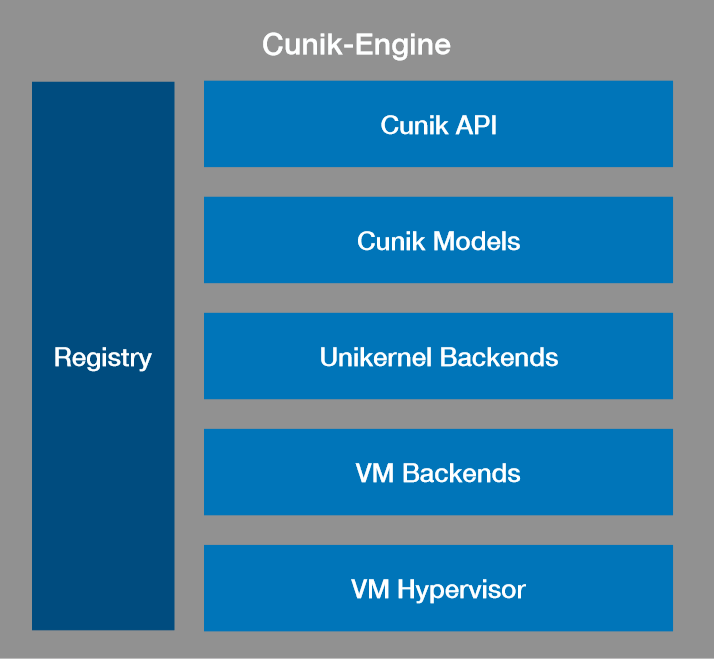
\includegraphics[width=0.5\linewidth]{pictures/resp1.png}
\caption{Cunik-engine 架构}
\end{figure}
其具体细节可参考
\href{https://github.com/OSH-2018/X-Doudou/tree/master/concluding-report}{X-Doudou文档}。
调用 Cunik 后,程序会执行如下的内容:

\begin{enumerate}
\item 用户通过调用 Cunik API 中的 Creat、Run、Stop、
Remove、Inspect 等 API 接口命令来启动 Cunik-engine。
\item Cunik-engine 在接受到命令后,首先会生成一个 Cunik
Config,用于生成 Cunik Object。
\item 通过Cunik Models,engine 会生成 Cunik Object,并加入到
Cunik Registry 中,或对已有 Cunik Object 进行运行状态的修改。
\item 然后,Unikernel Backends 会根据不同的 Cunik Object
选择不同的 Unikernel 实现方式。
\item 接下来,根据所选择的 Unikernel 实现方式,并在 Image Regsitry
中查询 Unikernel 应用的 image ,然后由 VM Backends 生成 VM Config。
\item VM Hypervisor 接收 VM Config 并选择合适的虚拟机来运行这个
Unikernel 应用。
\end{enumerate}

该项目目前只实现了对 kvm/qemu 虚拟机、Rumprun 和 OSv 两种 Unikernel 实现的简单支持。可以改进的内容包括:
\begin{itemize}
\item 整理当前 Cunik-engine 的架构;
\item 实现对更多虚拟机平台以及 Unikernel 实现的支持;
\item 持续支持新的 Unikernel 实现,并加入更多方便
镜像打包与应用部署的特性,使其能够满足生产环境的需要;
\item 更好的交互体验:实现在用户发出 Request 后,
自动为用户选择最合适的一系列 Cunik 应用,达成从前端到后端的一键式搭建服务。
\end{itemize}

\subsubsection{ X-zos 小组}\label{ssubsec:x-zos}

\paragraph{1. 项目简介}~\par

该项目设计了一个利用系统自带的虚拟网卡,通过socket和多线程
并发收发调试信息的日志式调试系统 Umonitor,为运维人员对
Unikernel的调试和维护工作提出了更为轻松有效的解决方案。用户在
使用时只需在每个需要调试的 Unikernel 里调用工具中的 \texttt{send\_log()}
函数,将想要得到的调试信息传入函数,然后在主机的环境里面启动一个host 端,host 端就能通过虚拟网卡接口接收到来自不同 Unikernel 的调试信息并整理保存。

关键词: Unikernel、调试

参考项目: Rumprun

\paragraph{2. 项目可行性分析}~\par
\begin{itemize}
\item 传统的调试手段在 Unikernel 上难以进行。包括:
    \begin{itemize}
    \item 通过与其他进程通信来进行追踪和调试\\
        Unikernel 为了实现精简,而放弃了原有的很多功能,
        其中就包括多进程切换。没有了多进程,就无法利用与其他进程通信来进行debug。
    \item 编程过程中将信息输出在控制台或者文件中\\
        在实际运行 Unikernel 的时候是不会模拟显示器的,
        所以无法将调试信息输出到控制台。又因为 Unikernal 的文件系统
        做了很大的精简,没有VFS,而且不同 Unikernal 的文件系统设计也
        不完全一样,所以,我们如果将日志写入文件,就很难再将虚拟磁盘中的东西读出来。
    \end{itemize}
\item Unikernel 采用了比较原始的单地址空间方式,这可以简化了调试的难度。
单地址空间有助于定位需要的信息在的位置,而并不会影响 Unikernel 的性能。
\end{itemize}
\paragraph{3. 项目困难点分析}~\par
\begin{itemize}
\item 可能实现的方案选择很多,包括文件I/O,串口通信,网络通信等。如何选择最合适的方案需要一定的时间与试错成本。本实验最终选择了通过网络完成unikernel向host发送日志信息的过程。
\end{itemize}

\paragraph{4. 项目成果分析}~\par

该小组设计的 Umonitor 已经可以在 rumpkernel 的平台上通过对
Unikernel 源代码的修改,通过网络通信的方式将 Unikernel 中我们
想要的调试信息输出到制定文件中,初期制定目标已经达到。项目的优势包括:

\begin{enumerate}
\item  \textbf{并发性}:只需启动一个host端就能服务复数的
Unikernel 而无需多开,提高了效率;
\item \textbf{兼容性}:避开了不同的 Unikernel 的差异性,如使用的语言,
内存空间,文件系统等的不同,选择了它们的共性,对 socket 的支持作为实现方法,
几乎所有的 Unikernel 都能无难度地移植这个调试系统;
\item \textbf{高度可控可定制化}:直接在运行 Unikernel 的虚拟机的模拟
vga 输出界面打印调试信息会造成很大的切换和检索的麻烦,而重定向 vga
输出信息至某个文件会输出非常多 Unikernel 自带对调试无用或者不够清晰的信息,
不能得到一个组织良好的日志文件。此外,多个 Unikernel 并发重定向在某些情况下
可能造成输出混杂,不能正确地输出文件。利用 socket 传递自己想要的调试信息并
组织保存,能够生成用户自己最需要的最有用的日志文件,提高调试的效率。
\end{enumerate}

项目可以改进的方向包括:
\begin{enumerate}
\item Unikernel 的调试工具必然需要提供一个通用的接口以实现
对不同种类 Unikernel 的支持。目前的 Umonitor 已经实现了能同时
对多个 Unikernel 的调试,所以下一步的目标可以是实现对多种 Unikernel 的通用接口。使其够方便的支持现阶段较为成熟的 Unikernel 实现的同时
也能够通过用户友好的配置界面对其他 Unikernel 进行支持。
\item Umonitor 在运行之后实际上仍然只能被动地接受被调试的 Unikernel
输出的调试信息,这样虽然能够在一次设置后找到对应的错误信息出现的位置,
但想要在 Unikernel 运行中途添加调试信息输出或者更进一步的设置断点和
逐句执行都还做不到。可以考虑添加交互式调试功能。
\end{enumerate}
\end{comment}

\section*{许可协议}
本文档以知识共享署名 4.0 国际 (CC BY 4.0)许可证发布。

\vspace{2ex}
\noindent\textbf{\large 您可以自由地}:
\begin{description}
\item[共享] 在任何媒介以任何形式复制、发行本作品;
\item[演绎] 修改、转换或以本作品为基础进行创作
在任何用途下,甚至商业目的。
\end{description}

\vspace{2ex}
\noindent\textbf{\large 惟须遵守下列条件}:
\begin{description}
\item[署名] 您必须给出适当的署名,提供指向本许可协议的链接,
同时标明是否(对原始作品)作了修改。您可以用任何合理的方式来署名,
但是不得以任何方式暗示许可人为您或您的使用背书。
\item[没有附加限制] 您不得使用法律术语或者技术措施,从而限制其他人
做许可协议允许的事情。
\end{description}

\vspace{2ex}
\noindent\textbf{\large 声明}:

您不必因为公共领域的作品要素而遵守许可协议,或者您的使用被可适用的例外或限制所允许。

不提供担保。许可协议可能不会给与您意图使用的所必须的所有许可。
例如,其他权利比如形象权、隐私权或人格权可能限制您如何使用作品。

本许可证的全文位于:\\
\centerline{\url{https://creativecommons.org/licenses/by/4.0/legalcode.zh-Hans}}


\begin{thebibliography}{99}
\bibitem{bib:os-concept} Abraham Silberschatz, Peter B. Galvin and Greg Gagne.
\textit{操作系统概念}[M]. 郑扣根, 唐杰, 李善平\ 译. 北京: 机械工业出版社, 2021: 54-58.

\bibitem{bib:docker-security-selinux} Daniel J Walsh. \texttt{Are Docker containers really secure?}[Z/OL]. Opensource.com, 2014 (20140622) [2022-04-10]. \url{https://opensource.com/business/14/7/docker-security-selinux}

\bibitem{bib:unikernel}
\textit{Unikernels: Rethinking Cloud Infrastructure}[Z/OL].
@unikernel [2022-02-18]. \url{https://web.archive.org/web/20220218194213/http://unikernel.org/}

\bibitem{bib:unikraft} Simon Kuenzer, Vlad-Andrei Bădoiu, Hugo Lefeuvre, Sharan Santhanam,
Alexander Jung, Gaulthier Gain, Cyril Soldani, Costin Lupu, \c{S}tefan Teodorescu, Costi Răducanu,
Cristian Banu, Laurent Mathy, Răzvan Deaconescu, Costin Raiciu and Felipe Huici.
\textit{Unikraft: Fast, Specialized Unikernels the Easy Way}[J/OL]. EuroSys '21, 2021, April: 26–29
[2022-03-27]. \url{https://dl.acm.org/doi/10.1145/3447786.3456248} \texttt{doi:10.1145/3447786.3456248}.

\bibitem{bib:unikernel-secuirty} Spencer Michaels and Jeff Dileo. \textit{Assessing Unikernel Security
}[R/OL]. Version 1.0. NCC Group, 2019: 4-10 [2022-03-27].
\url{https://research.nccgroup.com/wp-content/uploads/2020/07/ncc_group-assessing_unikernel_security.pdf}

\bibitem{bib:1-rust-lang} \textit{Rust Programming Language}[G/OL]. [2022-03-26]. \url{https://web.archive.org/web/20220326232949/https://www.rust-lang.org/}
\bibitem{bib:2-why-rust} @程序师视野. \textit{我们为什么要选择小众语言 Rust 来开发软件?}[Z/OL]. 程序师. [2017-06-26]. \url{https://web.archive.org/web/20170626061304/https://www.techug.com/post/why-we-choose-rust-to-dev.html}
\bibitem{bib:3-why-rust-pop}
Jake Goulding. \textit{What is Rust and why is it so popular?}[Z/OL]. Stack Overflow Blog. 2020 (20200120) [2022-03-24]. \url{https://web.archive.org/web/20220324021421/https://stackoverflow.blog/2020/01/20/what-is-rust-and-why-is-it-so-popular/}
\bibitem{bib:4-rust-go-cmp} CharyGao. \textit{也许是最客观、全面的比较 Rust 与 Go:都想把 Rust 也学一下}[Z/OL]. 博客园. 2020 (20201207) [2022-03-29]. \url{https://web.archive.org/web/20220329090604/https://www.cnblogs.com/Chary/p/14097609.html}
\bibitem{bib:5-why-rust2} 黄光星. \textit{为什么要使用 Rust 语言?Rust 语言的优势在哪里?}[Z/OL].
2020 (20200513) [2022-03-29] \url{https://www.zhihu.com/question/393796866}
\bibitem{bib:6-why-rust-pop-2} Krzysztof Wróbel. \textit{Rust programming language - what is rust used for and why is so popular?}[Z/OL]. codilime, 2022 (20220325) [2022-03-25]. \url{https://codilime.com/blog/why-is-rust-programming-language-so-popular/}
\bibitem{bib:7-rust-by-num} Pavan Belagatti.[\textit{Rust by the Numbers: The Rust Programming Language in 2021}[Z/OL]. The New Stack. 2021 (20210512) [2022-03-25]. \url{https://thenewstack.io/rust-by-the-numbers-the-rust-programming-language-in-2021/}
\bibitem{bib:8-rust-compatibility} \textit{Rust By Example}[M/OL]. Compatibility [2022-03-26]. \url{https://web.archive.org/web/20220326130141/https://doc.rust-lang.org/rust-by-example/compatibility.html}

\bibitem{bib:risc-v-manual} David Patterson and Andrew Waterman. \textit{RISC-V 手册: 一本开源指令集的指南}[S]. 勾凌睿, 黄成, 刘志刚译. 2018: 13-21
\bibitem{bib:riscv-support} Jeff Tranter. \textit{What is RISC-V and Why is it Important?}[Z/OL]. ICS. 2021 (20210512) [2022-03-27]. \url{https://www.ics.com/blog/what-risc-v-and-why-it-important}
\bibitem{bib:riscv-gcc} \textit{Using the GNU Compilers Collections (GCC)}[G/OL]. 2021: RISC-V Options [2022-03-27]. \url{https://gcc.gnu.org/onlinedocs/gcc-11.2.0/gcc/RISC-V-Options.html#RISC-V-Options}
\bibitem{bib:riscv-llvm} \textit{Clang command line argument reference: Clang 15.0.0git documentation}[G/OL]. 2022: RISCV [2022-03-27] \url{https://clang.llvm.org/docs/ClangCommandLineReference.html#riscv}
\bibitem{bib:riscv-linux} Drew Fustini. \textit{Linux on RISC-V
with Open Hardware}[Z/OL]. Embedded Linux Conference, 2020 [2022-03-27]. \url{https://elinux.org/images/3/3d/Linux_riscv_elce2020.pdf}
\bibitem{bib:riscv-debian} \textit{RISC-V}[G/OL]. Debian Wiki, 2022 (2022-03-24) [2022-03-27]. \url{https://wiki.debian.org/RISC-V?action=recall&rev=151}

\bibitem{bib:riscv-spec1} \textit{The RISC-V Instruction Set Manual
Volume I: Unprivileged ISA}[S/OL]. Editors Andrew Waterman and Krste Asanović. Version 2.1. RISC-V Foundation, 2019 (20191213) [2022-03-25]. \url{https://github.com/riscv/riscv-isa-manual/releases/download/Ratified-IMAFDQC/riscv-spec-20191213.pdf}
\bibitem{bib:riscv-spec2} \textit{The RISC-V Instruction Set Manual
Volume II: Privileged Architecture}[S/OL]. Editors Andrew Waterman, Krste Asanović and John Hauser.
Version 1.9.1. RISC-V International, 2021 (20211204) [2022-03-27]. \url{https://github.com/riscv/riscv-isa-manual/releases/download/Priv-v1.12/riscv-privileged-20211203.pdf}
\bibitem{bib:riscv-spec3} \textit{RISC-V Debug Support
}[S/OL]. Editors Ernie Edgar and Tim Newsome. Version 1.0.0-Stable. SiFive, Inc., 2022(20220209)[2022-03-27]. \url{https://github.com/riscv/riscv-debug-spec/raw/b659d7dc7f578e1a2a76f9e62a5eec0f2d80045c/riscv-debug-stable.pdf}
\bibitem{bib:riscv-spec4} \textit{RISC-V Processor Trace}[S/OL]. Gajinder Panesar and
Iain Robertson. Version 1.0. UltraSoC Technologies Ltd., 2020(20200320)[2022-03-27]. \url{https://github.com/riscv/riscv-trace-spec/raw/e372bd36abc1b72ccbff31494a73a862367cbb29/riscv-trace-spec.pdf}

\bibitem{bib:amd64-manual} \textit{AMD64 Architecture Programmer's Manual: Volumes 1-5}[S/OL]. Revision 4.04, Advanced Micro Devices, Inc., 2021 (202111) [2022-03-27]. \url{https://www.amd.com/system/files/TechDocs/40332.pdf}
\bibitem{bib:amd64-manual-intel} \textit{Intel\textsuperscript{®} 64 and IA-32 Architectures Software Developer’s Manual}[S/OL]. Order Number: 325462-076US, Intel Corporation, 2021 (202112) [2022-03-27]. \url{https://cdrdv2.intel.com/v1/dl/getContent/671200}

\bibitem{bib:armv8-reference} \textit{Arm\textsuperscript{®} Architecture Reference Manual
for A-profile architecture}[S/OL]. Version 21.0, Arm Limited, 2022 [2022-03-27]. \url{https://developer.arm.com/documentation/ddi0487/latest}

\bibitem{bib:12-clickos} Joao Martins, Mohamed Ahmed, Costin Raiciu, Vladimir Olteanu,
Michio Honda, Roberto Bifulco and Felipe Huici. \textit{ClickOS and the Art of Network Function Virtualization}[C/OL]. 11th USENIX Symposium on Networked Systems
Design and Implementation. Seattle: USENIX Association. 2014: 459-473[2022-03-22]. \url{http://cnp.neclab.eu/projects/clickos/clickos.pdf}
\bibitem{bib:13-clickos2} Joao Martins, Mohamed Ahmed, Costin Raiciu and Felipe Huici.
\textit{Enabling Fast, Dynamic Network Processing with ClickOS}[J/OL]. HotSDN'13, 2013, August: 67-72[2022-03-22]. \url{http://cnp.neclab.eu/projects/clickos/clickos-workshop.pdf}

\bibitem{bib:11-unikerel2} Anil Madhavapeddy and David J. Scott. \textit{Unikernels: Rise of the Virtual Library Operating System}[J/OL]. ACM Queue, 2014, 11 [2022-03-22].  \url{https://queue.acm.org/detail.cfm?id=2566628}

\bibitem{bib:9-includeos}  Bratterud et al. \textit{IncludeOS: A minimal, resource efficient unikernel for cloud systems}[G/OL]. Adrian Colyer, The morning paper: a random walk through Computer Science research. 2016 (20160222) [2022-03-22]. \url{https://blog.acolyer.org/2016/02/22/includeos}
\bibitem{bib:10-includeos2} Nur Hussein. \textit{IncludeOS: a unikernel for C++ applications}[Z/OL]. 2017 (20170725) [2022-03-22]. \url{https://lwn.net/Articles/728682/}

\bibitem{bib:14-rusty-hermit} \textit{RustyHermit - A Rust-based, lightweight unikernel}[G/OL]. rusty-hermit 0.3.10. [2022-03-25]. \url{https://docs.rs/crate/rusty-hermit/0.3.10}
%\bibitem{bib:15-rust-runtime} Jason 于航. \textit{Rust Runtime 与 ABI}[M/OL]. 知乎专栏, 2021 (20210509) [2022-03-25] \url{https://zhuanlan.zhihu.com/p/370897059}
%\bibitem{bib:16-rust-runtime2} \textit{The Rust runtime}[G/OL]. The Rust Reference. [2022-03-17].
%\url{https://web.archive.org/web/20220317124224/https://doc.rust-lang.org/reference/runtime.html}
\bibitem{bib:17-rusty-hermit2} @stlankes. \textit{The \texttt{RustyHermit} Unikernel}[Z/OL]. Rust OSDev. 2021 (20210122) [2022-03-25]. \url{https://rust-osdev.com/showcase/rusty-hermit/}

\bibitem{bib:18-intra-unikernel} Mincheol Sung and Pierre Olivier. \textit{Intra-Unikernel Isolation with Intel Memory Protection Keys}[C/OL]. 16th ACM SIGPLAN/SIGOPS International Conference on Virtual Execution Environments. Lausanne: Association for Computing Machinery, 2022. \texttt{doi:10.1145/3381052.3381326}.
\bibitem{bib:19-mpk} \textit{Memory Protection Keys}[G/OL]. The Linux Kernel, 5.17.0. [2022-03-18]. \url{https://web.archive.org/web/20220318143208/https://www.kernel.org/doc/html/latest/core-api/protection-keys.html}
%\bibitem{bib:20-linux-kernel} Huo的藏经阁. \textit{linux内核那些事之Memory protection keys(硬件原理)}[Z/OL]. CSDN博客. 2021 (20211119) [2022-03-25]. \url{https://blog.csdn.net/weixin_42730667/article/details/121386896}
\bibitem{bib:21-rump-kernel} Wikipedia Contributors. \textit{Rump kernel}[G/OL]. Wikipedia, 2021 (20210903) [2022-03-29]. \url{https://en.wikipedia.org/w/index.php?title=Rump_kernel&oldid=1042218732}
\bibitem{bib:22-xen} Antti Kantee. \textit{Xen on Rump Kernels and the Rumprun Unikernel}[Z/OL]. XenProject, 2015 (20150806) [2021-08-18].  \url{https://web.archive.org/web/20210818101601/https://xenproject.org/2015/08/06/on-rump-kernels-and-the-rumprun-unikernel/}

\bibitem{bib:23-mirageos} Mircea Cosbuc. \textit{All About Unikernels: Part 2, Two Different Approaches, MirageOS and Rumprun}[Z/OL]. Container Solutions, 2020 (20200125) [2022-01-27]. \url{https://web.archive.org/web/2021*/https://blog.container-solutions.com/all-about-unikernels-part-2-mirageos-and-rumprun}
\bibitem{bib:24-rumrun} Sebastian Wicki. \textit{The Rumprun Unikernel}[Z/OL]. pkgsrcCon, 2016
[2022-03-25]. \url{https://pkgsrc.org/pkgsrcCon/2016/rumprun.pdf}
\bibitem{bib:canary} Wikipedia contributors. \textit{Sentinel species}[G/OL]. Wikipedia, 2022 (20220319) [2022-03-24]. \url{https://en.wikipedia.org/w/index.php?title=Sentinel_species&oldid=1078038868}
\bibitem{bib:unikraft-secuirty} \textit{Unikraft's Inherent Security Benefits}[Z/OL]. Unikraft, 2022 [2022-03-29]. \url{https://web.archive.org/web/20220329100701/https://unikraft.org/docs/features/security/}
\bibitem{bib:rcore-os} Yu Chen and Yifan Wu. \textit{rCore Tutorial Book}[M/OL]. Version 3,
2022(20220102) [2022-03-27]. \url{https://rcore-os.github.io/rCore-Tutorial-Book-v3/chapter0/0intro.html}

\bibitem{bib:kata} \textit{Kata Containers - Open Source Container Runtime Software}[Z/OL].
Kata Containers, [2022-04-02]. \url{https://web.archive.org/web/20220402043101/https://katacontainers.io/}

\bibitem{bib:gvisor} \textit{gVisor}[Z/OL]. [2022-04-02]. \url{https://web.archive.org/web/20220402043121/https://gvisor.dev/}

\bibitem{bib:iot-sys} 刘于苇. \textit{与嵌入式RTOS大不同,主流物联网操作系统中哪款适合你?}[Z/OL].
电子工程专辑, 2021 (20210518) [2022-03-12]. \url{https://www.eet-china.com/news/202105180818.html}
\bibitem{bib:ms-rtos} ScilogyHunter. \textit{MS-RTOS正式发布啦!!!}[Z/OL]. CSDN, 2020 (20200716) [2022-03-12]. \url{https://blog.csdn.net/ScilogyHunter/article/details/107390947}
\bibitem{bib:rust-os-comparison} flosse, wmanley, ticki, et al. \textit{Rust OS comparison}[G/OL]. GitHub, 2022 (20220408) [2022-04-10]. \url{https://github.com/flosse/rust-os-comparison/tree/f3eb1aae4f080fafd81b44254f54e387ac5f6b9d}
\end{thebibliography}
\end{document}